%%%%%%%%%%%%%%%%%%%%%%%%%%%%%%%%%%%%%%%%%%%%%%%%%%%%%%%%%%%%%%%%

\chapter{Analyzing DC Circuits - Powerful Tools}

Electrical networks can be complicated. One might model a computer chip as an electrical network containing millions or billions of nodes and edges. In this chapter, we further develop our analysis tools to be able to handle more complicated circuits.
\par
The first two sections introduce algorithms that you, or a computer, could use to analyze a circuit. The third technique involves combining sources to simplify an otherwise complex circuit, while hopefully providing some intuitive insight about voltage and current sources. The fourth technique, superposition, transcends several engineering classes and will provide further insight into linear circuits, and engineering systems.
\par
\section{Nodal Analysis}
This section describes a method of analysis called Nodal Analysis. The basic strategy of this technique is to:
\begin{itemize}
\item Identify uniques nodes.
\item Create a variable to represent the voltage difference for each node with respect to a common reference point. For node A, this will be called $V_{A-Ref}$ or just shortened to $V_A$.
\item For each node write down $\Sigma I_{in}=0$. 
\end{itemize}

\subsection{Simple Example}
Let's try out this procedure for a simple example and work out the bugs.

\begin{figure}[H]
\begin{center}
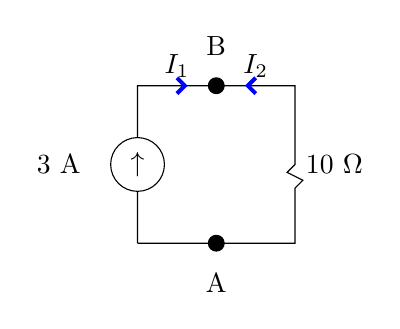
\begin{tikzpicture}
\draw (0,0)--(0,1)node[circle, draw=black, fill=white]{$\uparrow$}--(0,2)--(2,2)
--(2,1)--(1.9,.9)--(2.1,.8)--(2,.7)--(2,0)--(0,0);
\draw node at (-1,1) {3 A};
\draw node at (2.5,1) {10 $\Omega$};
\draw node at (1,2.5) {B};
\draw node at (1,-.5) {A};
\filldraw (1,2) circle[radius=1 mm];
\filldraw (1,0) circle[radius=1 mm];
\draw [draw=blue, line width=0.5mm] (.5,2.1)--(.6,2)--(.5,1.9);
\draw node at (.5,2.25) {$I_1$};
\draw [draw=blue, line width=0.5mm] (1.5,2.1)--(1.4,2)--(1.5,1.9);
\draw node at (1.5,2.25) {$I_2$};
\end{tikzpicture}
\caption{A simple nodal analysis example}
\end{center}
\end{figure}

Write $\Sigma I_{in}=0$ for each node. We have two nodes. We'll need to determine the current through resistors. Ohm's Law says that the current is the voltage \textbf{difference} across the resistor divided by the resistance. 
\par
\begin{align}
I_1+I_2=0 \rightarrow 3 + \frac{A-B}{10}=0&&\text{Node B} \label{E:4N}\\
-I_1-I_2=0 \rightarrow -3 + \frac{B-A}{10}=0&&\text{Node A} \notag 
\end{align} 

So far, so good - we have two equations and two unknowns. Our system of two equations looks like it should produce one solution. But look closely at the second equation, it is just the first equation multiplied by (-1)! The second equation is a duplicate of the first.\par

We really just have one equation and two unknowns. We would say that these two equations are not independant.\par

\begin{alevel}
Consider the following set of N equations and M unknowns. What are M and N?
\begin{align*}
3x+y&=10\\
x-y&=5\\
2x-5y&=8
\end{align*} 
\end{alevel}

\begin{blevel}
If you have one equation and two unknowns, how many solutions will you have? One? Infinite? None?
\end{blevel}

\begin{clevel}
Solve the following equation for x and y: (x+y=10). Report ALL solutions.
\end{clevel}

\begin{dlevel}
Suppose you have three equations and three unknowns. How can you tell if the third equation is just a combination of the other two?
\end{dlevel}

Let's continue with our example and solve for all possible combinations for the voltages at A and B.
\par
\begin{align*}
3 + \frac{A-B}{10}=0\tag{Node B}\\
30 = B-A\\
B = A+30&&\leftarrow \text{rearranged Node B equation}
\end{align*} 

So, A can be anything so long as B is 30V higher than A. Figure~\ref{F:4NS} shows some of the possible solutions:

\begin{figure}[H]
\begin{center}
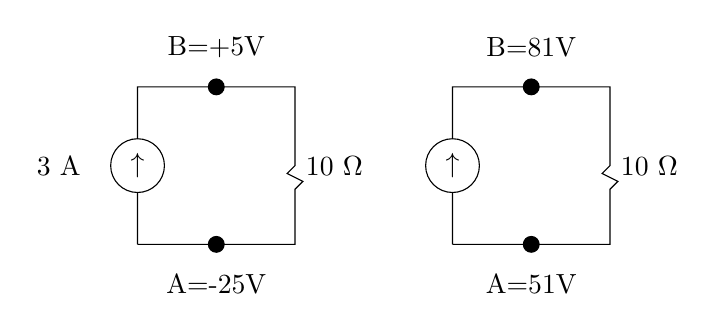
\begin{tikzpicture}
\draw (0,0)--(0,1)node[circle, draw=black, fill=white]{$\uparrow$}--(0,2)--(2,2)
--(2,1)--(1.9,.9)--(2.1,.8)--(2,.7)--(2,0)--(0,0);
\draw node at (-1,1) {3 A};
\draw node at (2.5,1) {10 $\Omega$};
\draw node at (1,2.5) {B=+5V};
\draw node at (1,-.5) {A=-25V};
\filldraw (1,2) circle[radius=1 mm];
\filldraw (1,0) circle[radius=1 mm];
%
\draw (4,0)--(4,1)node[circle, draw=black, fill=white]{$\uparrow$}--(4,2)--(6,2)
--(6,1)--(5.9,.9)--(6.1,.8)--(6,.7)--(6,0)--(4,0);
\draw node at (6.5,1) {10 $\Omega$};
\draw node at (5,2.5) {B=81V};
\draw node at (5,-.5) {A=51V};
\filldraw (5,2) circle[radius=1 mm];
\filldraw (5,0) circle[radius=1 mm];
\end{tikzpicture}
\caption{Two possible solutions for node voltages that satisfy Equation~\ref{E:4N}}
\label{F:4NS}
\end{center}
\end{figure}

Both are correct. There are an infinite number of solutions, but all solutions agree that the voltage DIFFERENCE from B to A is 30V.
\par
We can simplify things by requiring that we only present one of these solutions, one where one of the nodes is set to zero. In order words, we'll pick one of the nodes as the voltage reference point. Let's pick node A=0. Mathematically, this adds another equation (A=0). Our set of equations now looks like this:

\begin{align}
3 + \frac{A-B}{10}&=0\tag{Node B}\\
A&=0 \tag{Assign reference node}
\end{align} 

These equations are independent. Two independant equations with two variables leads to one solution. It wouldn't be hard to find a solution by substitution, but let's put the system of equations into matrix form and solve it that way. The matrix method works well when we have larger numbers of equations and unknowns.

\begin{align*}
\frac{1}{10}A-\frac{1}{10}B&=-3\\
A+0*B&=0
\end{align*}

\begin{align}
\left[ \begin{matrix}
\frac{1}{10} &	-\frac{1}{10}\\
1		&	0 \\
\end{matrix} \right]
\left[ \begin{matrix}
A\\
B\\
\end{matrix} \right]
=
\left[ \begin{matrix}
-3\\
0\\
\end{matrix} \right] \notag \\
M\vec{z}=\vec{b}
\end{align} 

Where M represesnts a 2x2 matrix\footnote{We usually employ the capitol letter A for this matrix, but because is one of the variables, I'm using M instead.}, z is the variable (with two parts, A and B), and b is the numerical term. To solve, find the inverse matrix for M and then apply it to both sides of the equation.

\begin{align}
M^{-1}M\vec{z}=M^{-1}\vec{b} \notag\\
\vec{z} = M^{-1}\vec{b}
\end{align} 

$M^{-1}$ can be found using a little linear algebra, google sheets, Matlab, or one of many other computational tools. In our case $M^{-1}$ turns out to be:


\begin{align*}
M^{-1}=\left[ \begin{matrix}
0 &	1\\
-10		&	1 \\
\end{matrix} \right]
\end{align*} 

\begin{blevel}
Multiply $M^{-1}$ by $\vec{b}$ to determine values for A and B. If you aren't familiar with matrix multiplication, look it up.
\end{blevel}

\begin{blevel}
The identity matrix, I, has all ones along the diagonal. Consider the 2x2 identity matrix multiplied by another generic 2x2 matrix as shown below. What do you get?

\begin{align*}
\left[ \begin{matrix}
1 &	0\\
0&	1 \\
\end{matrix} \right]*\left[ \begin{matrix}
a &	b\\
c&	d \\
\end{matrix} \right]=?
\end{align*} 
\end{blevel}

\begin{blevel}
Simplify $I^{5}$.
\end{blevel}

\begin{blevel}
Multiply $M^{-1}$ by M and see what you get. What this expected?
\end{blevel}

\begin{blevel}
Multiply $(M^{-1})^4$ by $M^5$. What do you get?
\end{blevel}

\begin{blevel}
Multiply this out:
\begin{align*}
\begin{vmatrix}0 &	1&2\\-10&1	&1 \\\end{vmatrix}
\begin{vmatrix}0 &	1\\-10&1\\ 2&3\\ \end{vmatrix}
\end{align*}
\end{blevel}

\begin{clevel}
When multiplying matrices together, there is a size rule. For example, you can multiply a 3x2 by a 2x7 matrix, but not a 2x7 by a 3x2. Describe the rule that determines if two matrices can be multiplied together?
\end{clevel}

\subsection{A more complex example}
Let's apply Nodal Analysis to a more complex problem.
\par
\begin{figure}[H]
\begin{center}
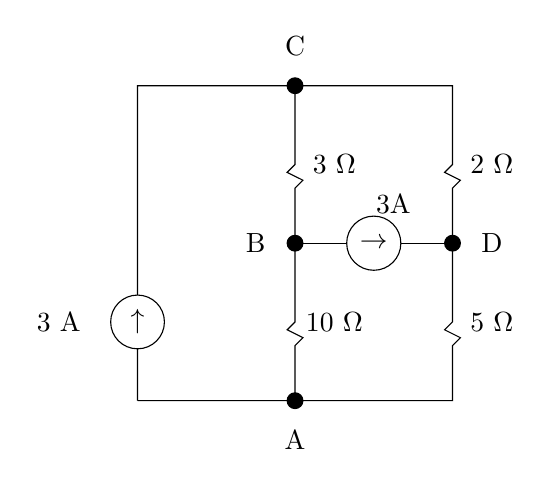
\begin{tikzpicture}
\draw (0,0)--(0,1)node[circle, draw=black, fill=white]{$\uparrow$}--(0,4)--(2,4)--(2,3)
--(1.9,2.9)--(2.1,2.8)--(2,2.7)--(2,2)--(2,1)
--(1.9,.9)--(2.1,.8)--(2,.7)--(2,0)--(0,0);
\draw (2,4)--(4,4)--(4,3)
--(3.9,2.9)--(4.1,2.8)--(4,2.7)--(4,2);
\draw (2,2)--(3,2)node[circle, draw=black, fill=white]{$\rightarrow$}--(4,2);
\draw node at (3.25,2.5) {3A};
\draw (4,2)--(4,1)
--(3.9,.9)--(4.1,.8)--(4,.7)--(4,0)--(2,0);
\draw node at (-1,1) {3 A};
\draw node at (2.5,1) {10 $\Omega$};
\draw node at (4.5,1) {5 $\Omega$};
\draw node at (2.5,3) {3 $\Omega$};
\draw node at (4.5,3) {2 $\Omega$};
\draw node at (1.5,2) {B};
\draw node at (2,-.5) {A};
\draw node at (2,4.5) {C};
\draw node at (4.5,2) {D};
\filldraw (2,4) circle[radius=1 mm];
\filldraw (2,2) circle[radius=1 mm];
\filldraw (4,2) circle[radius=1 mm];
\filldraw (2,0) circle[radius=1 mm];
\end{tikzpicture}
\caption{More complicated circuit for nodal analysis.}
\end{center}
\end{figure}

Let's make some observations:
\begin{enumerate}
\item There are four nodes, so we could write $\Sigma I_{in}=0$ four times. The last node, however, would not yield an independent equation. It would be a combination of the other three. We'll check that in a minute.

\item We will assign one node to be the reference node. Let's pick A.

\item We have four unknown node voltages (A,B,C and D) but since (A=0), we really only have three unknowns along with three meaningful (independent) node equations, plus $V_A=0$. We can count this as four unknown voltages and four unknown equations, or three equations and three unknowns if we just set A to 0.

\item After we write the equations, we move them into matrix form and solve.
\end{enumerate}

Writing the node equations:
\par
\begin{align}
\frac{C-B}{3}+\frac{0-B}{10}-3=0 &&\text{Node B}\notag\\
3 + \frac{B-C}{3}+\frac{D-C}{2}=0 &&\text{Node C}\notag\\
\frac{C-D}{2}+3+\frac{0-D}{5}=0 &&\text{Node D}
\end{align} 

Then, in matrix form:
\begin{align}
\left[ \begin{matrix}
(-\frac{1}{3}-\frac{1}{10})&	\frac{1}{3}&	0\\
\frac{1}{3}&	(-\frac{1}{3}-\frac{1}{2})&\frac{1}{2}\\
0	&	\frac{1}{2}&	(-\frac{1}{2}-\frac{1}{5})\\
\end{matrix} \right]
\left[ \begin{matrix}
B\\
C\\
D\\
\end{matrix} \right] =
\left[ \begin{matrix}
3\\
-3\\
-3\\
\end{matrix} \right]
\end{align}

\begin{blevel}
Determine $M^{-1}$ for this example.
\end{blevel}

\begin{clevel}
Determine the voltages B, C and D.
\end{clevel}

\begin{blevel}
Use your voltages for B and C to determine the current through the 3 Ohm resistor. Determine the power absorbed by the 3 Ohm resistor.
\end{blevel}

\begin{clevel}
Fill in the table indicating the power absorbed or produced by each component. Check that the power produced by the sources equals the power absorbed by the resistors. Remember, if current flows from - to + for a component, then that component is producing power.
\begin{table}[H]
\begin{center}
\begin{tabular}{|c|c|c|c|} \hline
component & I&$\Delta V$&power absorbed (- if produced) \\ \hline
3 $\Omega$ &&&	\\ \hline
2 $\Omega$&&&	\\ \hline
10 $\Omega$ &&&	\\ \hline
5 $\Omega$ &&&	\\ \hline
3A left source &&&	\\ \hline
3A center source &&&	\\ \hline
\end{tabular}
\caption{Power check}
\label{T:4PCheck}
\end{center}
\end{table}
\end{clevel}

\begin{clevel}
Suppose all the resistors were 10 $\Omega$. Adjust your matrix and redetermine the voltages B, C and D. If you only record your new values for B, C and D, that will be sufficient.
\end{clevel}

%%%%%%%%%%%%%%%%%%%%%%%%%%%%%%%%%%%%%%%%%%%%%%%%%%%%%%
\subsection{Nodal Analysis with a Voltage Source}
Now suppose we swap out one of the current sources for a voltage source as shown in Figure~\ref{F:4NODV}. This complicates things because we no longer know the current flowing from A to D.

\begin{figure}[H]
\begin{center}
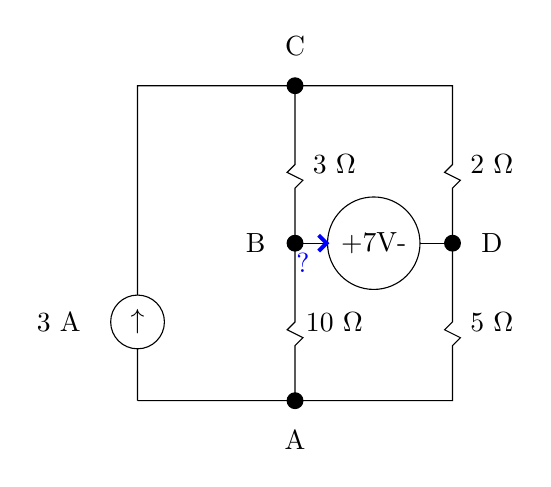
\begin{tikzpicture}
\draw (0,0)--(0,1)node[circle, draw=black, fill=white]{$\uparrow$}--(0,4)--(2,4)--(2,3)
--(1.9,2.9)--(2.1,2.8)--(2,2.7)--(2,2)--(2,1)
--(1.9,.9)--(2.1,.8)--(2,.7)--(2,0)--(0,0);
\draw (2,4)--(4,4)--(4,3)
--(3.9,2.9)--(4.1,2.8)--(4,2.7)--(4,2);
\draw (2,2)--(3,2)node[circle, draw=black, fill=white]{+7V-}--(4,2);
\draw [draw=blue, line width=0.5mm] (2.3,2.1)--(2.4,2)--(2.3,1.9);
\draw [text=blue] node at (2.1,1.75) {?};
\draw (4,2)--(4,1)
--(3.9,.9)--(4.1,.8)--(4,.7)--(4,0)--(2,0);
\draw node at (-1,1) {3 A};
\draw node at (2.5,1) {10 $\Omega$};
\draw node at (4.5,1) {5 $\Omega$};
\draw node at (2.5,3) {3 $\Omega$};
\draw node at (4.5,3) {2 $\Omega$};
\draw node at (1.5,2) {B};
\draw node at (2,-.5) {A};
\draw node at (2,4.5) {C};
\draw node at (4.5,2) {D};
\filldraw (2,4) circle[radius=1 mm];
\filldraw (2,2) circle[radius=1 mm];
\filldraw (4,2) circle[radius=1 mm];
\filldraw (2,0) circle[radius=1 mm];
\end{tikzpicture}
\caption{Current source replaced with voltage source. The current is no longer known.}
\label{F:4NODV}
\end{center}
\end{figure}

We can handle this unknown current by introducing a variable for this unknown current,\footnote{There are other approaches. One approach uses something called supernodes. We might cover it in class, or you might look it up if interested.} call it $I_1$.  Because we introduced another unknown, we need another equation (a bonus equation, if you will). \par
This bonus equation must take into account the information about the voltage source that hasn't yet been considered. The voltage source forces node B to be 7V greater than node D, or $B =D+7$.\par
Our equations look like this:
\
\begin{align}
\frac{C-B}{3}+\frac{0-B}{10}-I_1=0 \tag{Node B}\\
3 + \frac{B-C}{3}+\frac{D-C}{2}=0 \tag{Node C}\\
\frac{C-D}{2}+I_1+\frac{0-D}{5}=0 \tag{Node D}\\
B=D+7 \tag{Bonus Equation due to 7V Voltage Source}
\end{align} 

\begin{clevel}
Put this in matrix form and solve for the voltages at B, C and D. Just answers are sufficient.
\end{clevel}

\begin{alevel}
When doing nodal analysis, is it easier to handle a current source or a voltage source?
\end{alevel}

\begin{clevel}
Replace the other 3A current source with a 3V voltage source (positive side on top). Adjust your analysis accordingly. Write down the new matrix formulation and solve for the voltages at B, C and D.
\end{clevel}

\begin{clevel}
A circuit has 3 voltage sources and 9 nodes. If you follow the above approach, how many rows will the matrix M have?
\end{clevel}

\begin{clevel}
A circuit has 3 voltage sources, 5 current sources and 25 nodes. If you follow the above approach, how many rows will the matrix M have?
\end{clevel}


%%%%%%%%%%%%%%%%%%%%%%%%%%%%%%%%%%%%%%%%%%%%%%%%%%%%%%%%%%%%%%%%%%
\section{Loop Analysis}
Loop analysis is an alternative to nodal analysis. It is based on the idea that the sum of the voltages around any loop add to zero. Sometimes loop analysis is slower, sometimes faster. Sometimes it's more intuitive, sometimes not. It's good to have both tools, just like it pays to have multiple driving routes to your home. If one route closes or has bad weather, you can try the other one.\\

The premise behind loop analysis is to write KVL \footnote{The sum of the voltages around a loop is zero.} for \emph{some} of the loops in the circuit. If we pick the loops carefully, we can avoid duplicate equations and arrive with a solvable set of independent equations.
\par
Our first step is to consider how many loops a circuit might have.
\begin{alevel}
How many rectangles can be found in Figure~\ref{F:4RECT}?
\end{alevel}

\begin{blevel}
How many polygons can be found in Figure~\ref{F:4RECT}?
\end{blevel}

\begin{clevel}
How many polygons \textbf{that do not have any smaller polygons inside them} can be found in Figure~\ref{F:4RECT}?
\end{clevel}

\begin{figure}[H]
\begin{center}
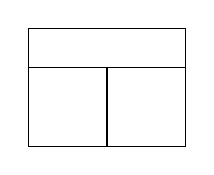
\begin{tikzpicture}
\draw (0,0)--(0,1.5)--(2,1.5)--(2,0)--(0,0);
\draw (0,1)--(2,1) (1,1)--(1,0);
\end{tikzpicture}
\caption{Fun box problem.}
\label{F:4RECT}
\end{center}
\end{figure}

Figure~\ref{F:4R} shows an electric circuit that is similar in structure to Figure~\ref{F:4RECT} (rotated 90 degrees).

\begin{figure}[H]
\begin{center}
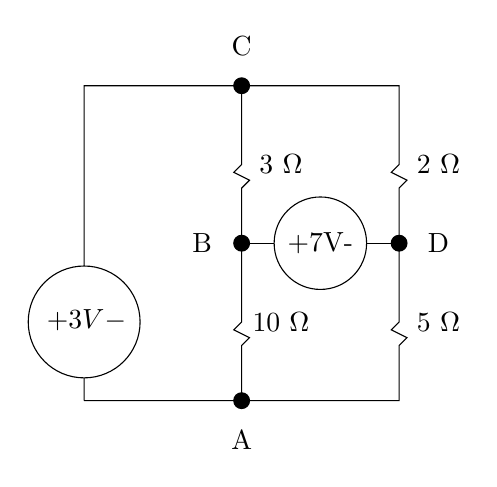
\begin{tikzpicture}
\draw (0,0)--(0,1)node[circle, draw=black, fill=white]{$\begin{matrix}+\\3V\\-\end{matrix}$}--(0,4)--(2,4)--(2,3)
--(1.9,2.9)--(2.1,2.8)--(2,2.7)--(2,2)--(2,1)
--(1.9,.9)--(2.1,.8)--(2,.7)--(2,0)--(0,0);
\draw (2,4)--(4,4)--(4,3)
--(3.9,2.9)--(4.1,2.8)--(4,2.7)--(4,2);
\draw (2,2)--(3,2)node[circle, draw=black, fill=white]{+7V-}--(4,2);
\draw (4,2)--(4,1)
--(3.9,.9)--(4.1,.8)--(4,.7)--(4,0)--(2,0);
\draw node at (2.5,1) {10 $\Omega$};
\draw node at (4.5,1) {5 $\Omega$};
\draw node at (2.5,3) {3 $\Omega$};
\draw node at (4.5,3) {2 $\Omega$};
\draw node at (1.5,2) {B};
\draw node at (2,-.5) {A};
\draw node at (2,4.5) {C};
\draw node at (4.5,2) {D};
\filldraw (2,4) circle[radius=1 mm];
\filldraw (2,2) circle[radius=1 mm];
\filldraw (4,2) circle[radius=1 mm];
\filldraw (2,0) circle[radius=1 mm];
\end{tikzpicture}
\caption{Example for loop analysis}
\label{F:4R}
\end{center}
\end{figure}

We will pick our loops such that no loops contain any other loops\footnote{This description works for planar circuits, circuits that can be drawn on 2D paper without criss-crossing wires.}. This circuit contains three such loops.\par
For each loop, we define a current ($I_1$,$I_2$ and $I_3$), and define that current always in the clockwise direction. If you really like misery, you could define some clockwise and some counterclockwise, track them all carefully and still make it work. \footnote{That would be like storing your driver's license in a recycling bin - I can't stop you.}

\begin{figure}[H]
\begin{center}
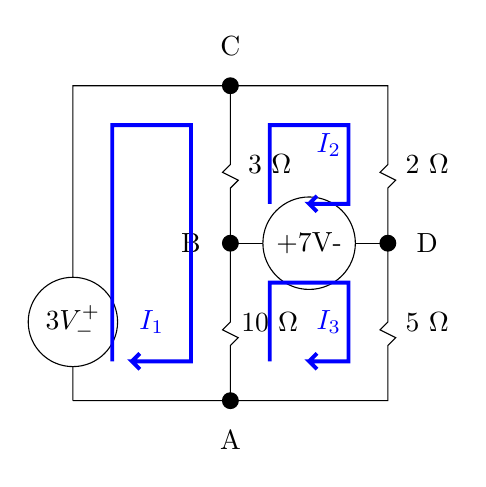
\begin{tikzpicture}
\draw (0,0)--(0,1)node[circle, draw=black, fill=white]{$3V_{-}^{+}$}--(0,4)--(2,4)--(2,3)
--(1.9,2.9)--(2.1,2.8)--(2,2.7)--(2,2)--(2,1)
--(1.9,.9)--(2.1,.8)--(2,.7)--(2,0)--(0,0);
\draw (2,4)--(4,4)--(4,3)
--(3.9,2.9)--(4.1,2.8)--(4,2.7)--(4,2);
\draw (2,2)--(3,2)node[circle, draw=black, fill=white]{+7V-}--(4,2);
\draw (4,2)--(4,1)
--(3.9,.9)--(4.1,.8)--(4,.7)--(4,0)--(2,0);
\draw node at (2.5,1) {10 $\Omega$};
\draw node at (4.5,1) {5 $\Omega$};
\draw node at (2.5,3) {3 $\Omega$};
\draw node at (4.5,3) {2 $\Omega$};
\draw node at (1.5,2) {B};
\draw node at (2,-.5) {A};
\draw node at (2,4.5) {C};
\draw node at (4.5,2) {D};
\filldraw (2,4) circle[radius=1 mm];
\filldraw (2,2) circle[radius=1 mm];
\filldraw (4,2) circle[radius=1 mm];
\filldraw (2,0) circle[radius=1 mm];
\draw [draw=blue, line width=0.5mm] (.5,.5)--(.5,3.5)--(1.5,3.5)
--(1.5,.5)--(.75,.5)--(.85,.4)--(.75,.5)--(.85,.6);
\draw [text=blue] node at (1,1) {$I_1$};
\draw [draw=blue, line width=0.5mm] (2.5,2.5)--(2.5,3.5)--(3.5,3.5)
--(3.5,2.5)--(3,2.5)--(3.1,2.4)--(3,2.5)--(3.1,2.6);
\draw [text=blue] node at (3.25,3.25) {$I_2$};
\draw [draw=blue, line width=0.5mm] (2.5,.5)--(2.5,1.5)--(3.5,1.5)
--(3.5,.5)--(3,.5)--(3.1,.4)--(3,.5)--(3.1,.6);
\draw [text=blue] node at (3.25,1) {$I_3$};
\end{tikzpicture}
\caption{Loops indicated in blue. Each loop has a current through it.}
\end{center}
\end{figure}

Note that the total current through the interior edges are combinations of these loop currents. For example, the current up through the $3 \Omega$ resistor is $I_2-I_1$.\par

Next, write KVL for each loop. There are two tricky parts to this.
\begin{itemize}
\item \textbf{First Tricky Thing:} Getting the signs right. More around each loop in clockwise direction. If you move from - to +, then add that voltage. If you move from + to - then subtract it. Recall that positive currents flow through resistors from + to -.
\item \textbf{Second Tricky Thing:} Handling components that have more than one loop current passing through it. The 3 Ohm resistor, for example, has $I_1$ passing through it from C to B and $I_2$ passing through it the other direction from B to C.
\end{itemize}

Write out KVL for each loop:
\begin{align*}
\text{First Loop (A-C-B-A):}&&+3-3(I_1-I_2)-10(I_1-I_3)&=0\\
\text{Second Loop (B-C-D-B):}&&-3(I_2-I_1)-2I_2+7V&=0\\
\text{Third Loop (A-B-D-A):}&&-10(I_3-I_1)-7V-5I_3&=0
\end{align*}

Put this in matrix form:
\begin{align}
\left[ \begin{matrix}
(-3-10)&	3&	10\\
3&	(-3-2)&0\\
10	&	0&	(-10-5)\\
\end{matrix} \right]
\left[ \begin{matrix}
I_1\\
I_2\\
I_3\\
\end{matrix} \right] =
\left[ \begin{matrix}
-3\\
-7\\
7\\
\end{matrix} \right]
\end{align}

\begin{blevel}
Determine the inverse of this matrix and write it down.
\end{blevel}

\begin{clevel}
Solve for the currents $I_1,I_2,I_3$.
\end{clevel}

\begin{clevel}
Suppose the direction of the 7V source were switched. Modify your equations and matrix and resolve for $I_1,I_2,I_3$.
\end{clevel}

\begin{dlevel}
Let's call the 7V source, $V_A$ and the 3V source, $V_B$. Why does the $V_A$ appear twice in on the right side of the equation while $V_B$ only appears once? Can $V_A$ appear three times? What assumptions have you made?
\end{dlevel}

\begin{dlevel}
What would happen to the algebra if we used all possible loops instead of just the loops that don't contain other loops?
\end{dlevel}

%%%%%%%%%%%%%%%%%%%%%%%%%%%%%%%%%%%%%%%%%%%%%%%%%
\subsection{Loop Analysis with Current Sources}
In this section, we will replace the 7V source with a 3A current source. This causes just a little trouble because we no longer know the voltage from B to D. No worries - just assign it a variable, like $V_1$ \footnote{Do you see the similarity to nodal analysis?}. 
\par
But, we now have one too many unknowns. We need another equation. Solution: We can use information about what the current source is doing. The current source is forcing the current from B to D to be 3A. That current from B to D is $I_3-I_2$, so we can write $I_3-I_2=3 A$.

\begin{figure}[H]
\begin{center}
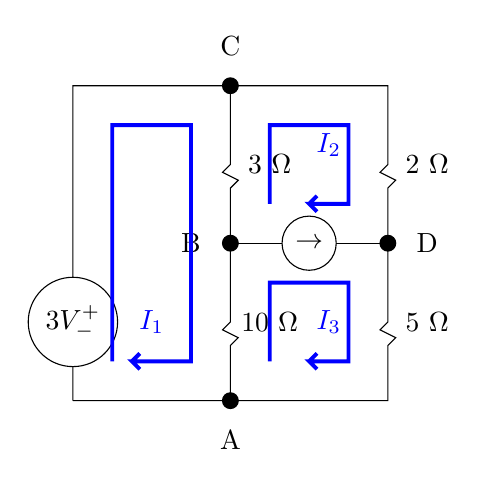
\begin{tikzpicture}
\draw (0,0)--(0,1)node[circle, draw=black, fill=white]{$3V_{-}^{+}$}--(0,4)--(2,4)--(2,3)
--(1.9,2.9)--(2.1,2.8)--(2,2.7)--(2,2)--(2,1)
--(1.9,.9)--(2.1,.8)--(2,.7)--(2,0)--(0,0);
\draw (2,4)--(4,4)--(4,3)
--(3.9,2.9)--(4.1,2.8)--(4,2.7)--(4,2);
\draw (2,2)--(3,2)node[circle, draw=black, fill=white]{$\rightarrow$}--(4,2);
\draw (4,2)--(4,1)
--(3.9,.9)--(4.1,.8)--(4,.7)--(4,0)--(2,0);
\draw node at (2.5,1) {10 $\Omega$};
\draw node at (4.5,1) {5 $\Omega$};
\draw node at (2.5,3) {3 $\Omega$};
\draw node at (4.5,3) {2 $\Omega$};
\draw node at (1.5,2) {B};
\draw node at (2,-.5) {A};
\draw node at (2,4.5) {C};
\draw node at (4.5,2) {D};
\filldraw (2,4) circle[radius=1 mm];
\filldraw (2,2) circle[radius=1 mm];
\filldraw (4,2) circle[radius=1 mm];
\filldraw (2,0) circle[radius=1 mm];
\draw [draw=blue, line width=0.5mm] (.5,.5)--(.5,3.5)--(1.5,3.5)
--(1.5,.5)--(.75,.5)--(.85,.4)--(.75,.5)--(.85,.6);
\draw [text=blue] node at (1,1) {$I_1$};
\draw [draw=blue, line width=0.5mm] (2.5,2.5)--(2.5,3.5)--(3.5,3.5)
--(3.5,2.5)--(3,2.5)--(3.1,2.4)--(3,2.5)--(3.1,2.6);
\draw [text=blue] node at (3.25,3.25) {$I_2$};
\draw [draw=blue, line width=0.5mm] (2.5,.5)--(2.5,1.5)--(3.5,1.5)
--(3.5,.5)--(3,.5)--(3.1,.4)--(3,.5)--(3.1,.6);
\draw [text=blue] node at (3.25,1) {$I_3$};
\end{tikzpicture}
\caption{Loop analysis with a current source}
\end{center}
\end{figure}

\begin{clevel}
Write down the modified set of equations with the current source described above. Put it in matrix form. Solve for $I_1,I_2,I_3, V_1$.
\end{clevel}

\begin{clevel}
A circuit has more voltage sources than current sources. Knowing nothing else, do you think it would be easier to use loop analysis or nodal analysis? 
\end{clevel}


\begin{clevel}
A circuit has the structure shown in figure. It contains 2 voltage sources and 1 current source. How many equations will be produced by the loop analysis method? 

\begin{figure}[H]
\begin{center}
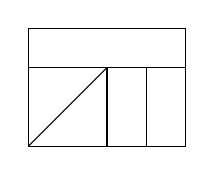
\begin{tikzpicture}
\draw (0,0)--(0,1.5)--(2,1.5)--(2,0)--(0,0);
\draw (0,1)--(2,1) (1,1)--(1,0);
\draw (0,0)--(1,1);
\draw (1.5,1)--(1.5,0);
\end{tikzpicture}
\caption{Circuit structure.}
\label{F:4RECT2}
\end{center}
\end{figure}

\end{clevel}
%%%%%%%%%%%%%%%%%%%%%%%%%%%%%%%%%%%%%%%%%%%%%%%%%%%%%%%%%%
\section{Source Transformations}
Earlier in this book, we simplified circuits by combining series or parallel connections of resistors. In this section, we'll get even more serious about simplication. We'll see that we can transform voltage sources into equivalent current sources and visa versa. By transforming sources at our convenience we can then combine parallel sets of current sources or series combinations of voltage sources.\par
First, though, we need to broaden our model of a voltage source.

\subsection{Improved model of a Voltage Source}
Consider an ideal voltage source connected to a resistor as shown in Figure~\ref{F:4RVA}:

\begin{figure}[H]
\begin{center}
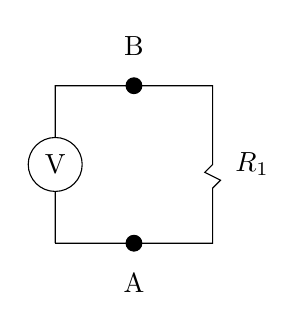
\begin{tikzpicture}
\draw (0,0)--(0,1)node[circle, draw=black, fill=white]{V}--(0,2)--(2,2)
--(2,1)--(1.9,.9)--(2.1,.8)--(2,.7)--(2,0)--(0,0);
\draw node at (2.5,1) {$R_1$};
\draw node at (1,2.5) {B};
\draw node at (1,-.5) {A};
\filldraw (1,2) circle[radius=1 mm];
\filldraw (1,0) circle[radius=1 mm];
\end{tikzpicture}
\caption{Ideal voltage source connected to a resistive load.}
\label{F:4RVA}
\end{center}
\end{figure}

The current through $R_1$ would be $\frac{V}{R_1}$. If $R_1$ were small, this current would get very big. If $R_1$ were infinitely small, the current would get infinitely big. \par
But this can't happen - there aren't any voltage sources that can deliver infinitely large current. Currents cause magnetic fields. An infinite current would cause an infinitely large magnetic field. If that doesn't impress you, the power consumed would also be infinite.

\begin{blevel}
What would be the magnetic field a distance of 3 cm away from a wire carrying 5A of current?
\end{blevel}

\begin{clevel}
For the circuit shown in Figure~\ref{F:4RVA}, with voltage V and resistance $R_1$, determine the power absorbed by the resistor as a function of V and $R_1$ only. What happens to the power absorbed in the $\lim_{R_1 \to 0}$? 
\end{clevel}

To make a better model \footnote{I say \emph{``better model"} because these are all approximate models, some better than others.} of a voltage source, we might add a resistor in series with the ideal voltage source. Maybe this resistance models some metal inside the box, or maybe a contact at the edge, but it also models any effect that tends to limit the amount of current that the source can produce.
\par
Our new model looks like Figure~\ref{F:4RVB}.

\begin{figure}[H]
\begin{center}
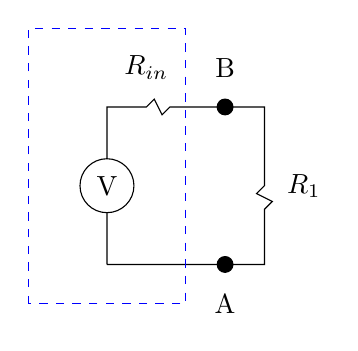
\begin{tikzpicture}
\draw (0,0)--(0,1)node[circle, draw=black, fill=white]{V}--(0,2)
--(.5,2)--(.6,2.1)--(.7,1.9)--(.8,2)
--(2,2)--(2,1)--(1.9,.9)--(2.1,.8)--(2,.7)--(2,0)--(0,0);
\draw node at (2.5,1) {$R_1$};
\draw node at (0.5,2.5) {$R_{in}$};
\draw node at (1.5,2.5) {B};
\draw node at (1.5,-.5) {A};
\draw [dashed, draw=blue] (-1,-.5)--(-1,3)--(1,3)--(1,-.5)--(-1,-.5);
\filldraw (1.5,2) circle[radius=1 mm];
\filldraw (1.5,0) circle[radius=1 mm];
\end{tikzpicture}
\caption{Real voltage source connected to a resistive load. The blue dashed box indicates the voltage source.}
\label{F:4RVB}
\end{center}
\end{figure}

\begin{blevel}
What is the current through $R_1$ in the $\lim_{R_1 \to 0}$? 
\end{blevel}

\begin{blevel}
Suppose $R_1$ were 50 $\Omega$. What would be the voltage across $R_1$ if the voltage source were a 9V battery with 7 $\Omega$ of internal resistance?  
\end{blevel}

\begin{blevel}
What is the voltage across $R_1$ in terms of V, $R_1$ and $R_{in}$? 
\end{blevel}

\begin{clevel}
Find the power absorbed by $R_1$ as a function of $R_{in}$ and V. What value of $R_1$, in terms of $R_{in}$, will result in the maximum amount of power absorbed by $R_1$? Hint: can you use calculus to determine the maximum of a function?
\end{clevel}

%%%%%%%%%%%%%%%%%%%%%%%%%%%%%%%%%
\subsection{Equivalent Sources}
Suppose we have a mysterious box - maybe someone claims its a voltage source, maybe not. We make some measurements to try to learn about what's inside the box. 

\begin{figure}[H]
\begin{center}
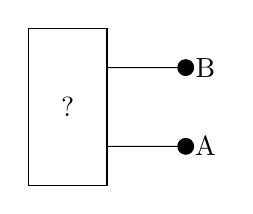
\begin{tikzpicture}
\draw (0,0) rectangle node{?} (1,2);
\draw node at (2.25,1.5) {B};
\draw node at (2.25,.5) {A};
\filldraw (1,1.5)--(2,1.5) circle[radius=1 mm];
\filldraw (1,.5)--(2,.5) circle[radius=1 mm];
\end{tikzpicture}
\caption{Mysterious box}
\end{center}
\end{figure}

First, we measure the voltage from A to B. We get 5V. Then we connect an ammeter between B and A and get 1A. We conclude that the black box could be the following:
\par
\begin{figure}[H]
\begin{center}
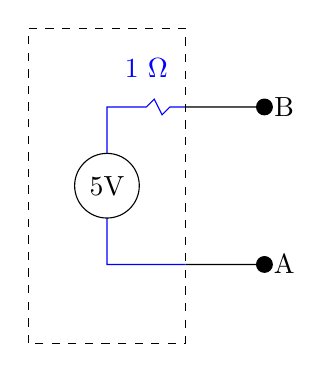
\begin{tikzpicture}
\draw [draw=blue] (1,0)--(0,0)--(0,1)node[circle, draw=black, fill=white]{5V}--(0,2)
--(.5,2)--(.6,2.1)--(.7,1.9)--(.8,2)--(1,2);
\draw node[text=blue] at (0.5,2.5) {1 $\Omega$};
\draw [dashed] (-1,-1) rectangle node{} (1,3);
\draw node at (2.25,2) {B};
\draw node at (2.25,0) {A};
\filldraw (1,2)--(2,2) circle[radius=1 mm];
\filldraw (1,0)--(2,0) circle[radius=1 mm];
\end{tikzpicture}
\caption{Mysterious box guess.}
\label{F:4TH}
\end{center}
\end{figure}

Ammeters act like a shorts, so the measured current would be 1A. Voltmeters act like open circuits, so there would be no current through the internal 1 $\Omega$ resistor and therefore no voltage drop across it. The voltmeter would read 5V.

\begin{figure}[H]
\begin{center}
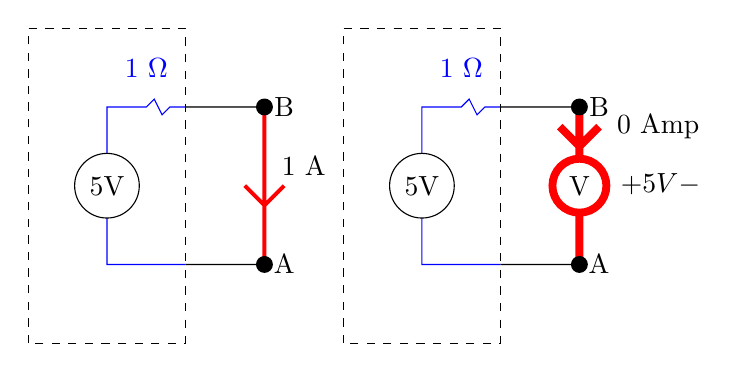
\begin{tikzpicture}
\draw [draw=blue] (1,0)--(0,0)--(0,1)node[circle, draw=black, fill=white]{5V}--(0,2)
--(.5,2)--(.6,2.1)--(.7,1.9)--(.8,2)--(1,2);
\draw node[text=blue] at (0.5,2.5) {1 $\Omega$};
\draw [dashed] (-1,-1) rectangle node{} (1,3);
\draw node at (2.25,2) {B};
\draw node at (2.25,0) {A};
\draw [draw=red, line width=0.5mm](2,2)--(2,0) (1.75,1)--(2,0.75)--(2.25,1);
\draw node at (2.5,1.25) {1 A};
\filldraw (1,2)--(2,2) circle[radius=1 mm];
\filldraw (1,0)--(2,0) circle[radius=1 mm];

\draw [draw=blue] (5,0)--(4,0)--(4,1)node[circle, draw=black, fill=white]{5V}--(4,2)
--(4.5,2)--(4.6,2.1)--(4.7,1.9)--(4.8,2)--(5,2);
\draw node[text=blue] at (4.5,2.5) {1 $\Omega$};
\draw [dashed] (3,-1) rectangle node{} (5,3);
\draw node at (6.25,2) {B};
\draw node at (6.25,0) {A};
\draw [draw=red, line width=1mm](6,2)--(6,1)node[circle, draw=red, fill=white]{V}--(6,0) (5.75,1.75)--(6,1.5)--(6.25,1.75);
\draw node at (7,1.75) {0 Amp};
\filldraw (5,2)--(6,2) circle[radius=1 mm];
\filldraw (5,0)--(6,0) circle[radius=1 mm];
\draw node at (7,1){$\begin{matrix}+\\5V\\-\end{matrix}$};
\end{tikzpicture}
\caption{Current measurement (left) and voltage measurement (right).}
\label{F:4TH2}
\end{center}
\end{figure}
\par
But the circuit in Figure~\ref{F:NotSpecial} would also work, an ammeter connected from B to A would read 1A and a voltmeter would read 5V.
\par
\begin{figure}[H]
\begin{center}
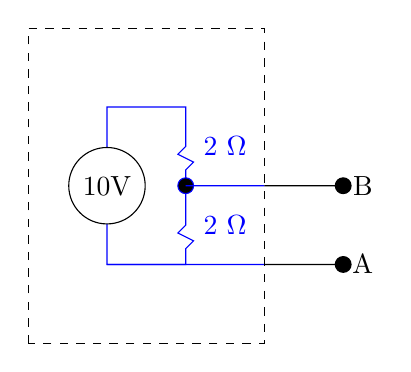
\begin{tikzpicture}
\draw [draw=blue] (1,0)--(-1,0)--(-1,1)node[circle, draw=black, fill=white]{10V}--(-1,2)--(0,2)--(0,1.5)--(-.1,1.4)--(.1,1.3)--(0,1.2)--(0,1);
\draw [draw=blue] (0,1)--(0,.5)--(-.1,.4)--(.1,.3)--(0,.2)--(0,0)--(-1,0);
\draw node[text=blue] at (.5,1.5) {2 $\Omega$};
\draw node[text=blue] at (.5,0.5) {2 $\Omega$};
\draw [dashed] (-2,-1) rectangle node{} (1,3);
\draw node at (2.25,1) {B};
\draw node at (2.25,0) {A};
\filldraw [draw=blue] (0,1) circle[radius=1 mm]--(1,1);
\filldraw (1,1)--(2,1) circle[radius=1 mm];
\filldraw (1,0)--(2,0) circle[radius=1 mm];
\end{tikzpicture}
\caption{A second option for the contents of the mysterious Box.}
\label{F:NotSpecial}
\end{center}
\end{figure}

Now here comes a surprising claim:\\
\\
\noindent
\textbf{Claim:} These two mystery implementations (Figure~\ref{F:NotSpecial} and Figure~\ref{F:4TH}) will produce the same voltages and currents no matter what combination of resistors, voltages, current sources, and multimeters connect to A and B \footnote{Outside the box. Inside the box, things will be different.}. This is a version of what is often credited as \textbf{Thev\'enin's Theorem}.

\begin{alevel}
If a resistor, R, were connect from B to A on the outside of the box for for Figure~\ref{F:4TH}, what would be the current through that resistor (in terms of R)?
\end{alevel}

\begin{clevel}
Suppose a resistor, R, were connected from B to A on the outside of the box for Figure~\ref{F:NotSpecial} what would be the current through that resistor (in terms of R)?
\end{clevel}

Figure~\ref{F:4NOR} shows another version for our black box. Let's find values so that it also behaves like the other circuits.

\begin{figure}[H]
\begin{center}
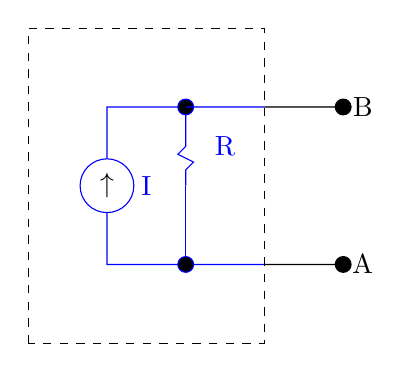
\begin{tikzpicture}
\draw [draw=blue] (1,0)--(-1,0)--(-1,1)node[circle, draw=blue, fill=white]{$\uparrow$}--(-1,2)--(0,2)--(0,1.5)--(-.1,1.4)--(.1,1.3)--(0,1.2)--(0,1);
\draw [draw=blue] (0,1)--(0,0)--(-1,0);
\draw node[text=blue] at (.5,1.5) {R};
\draw node[text=blue] at (-.5,1) {I};
\draw [dashed] (-2,-1) rectangle node{} (1,3);
\draw node at (2.25,2) {B};
\draw node at (2.25,0) {A};
\filldraw [draw=blue] (0,0) circle[radius=1 mm];
\filldraw [draw=blue] (0,2) circle[radius=1 mm]--(1,2);
\filldraw (1,2)--(2,2) circle[radius=1 mm];
\filldraw (1,0)--(2,0) circle[radius=1 mm];
\end{tikzpicture}
\caption{Circuit Z. Norton Equivalent. Current Source Version}
\label{F:4NOR}
\end{center}
\end{figure}

\begin{table}[H]
\begin{center}
\begin{tabular}{|c|c|p{60mm}|} \hline
Requirement & Conclusion & Reasoning \\ \hline
Voltmeter reads 5V & IR=5V & The volt-meter measures the voltage across the resistor. \\ \hline
Ammeter reads 1A & I=1A	& Since ammeters have little resistance, all the current will flow through the ammeter. Therefore, the current source must be 1A. \\ \hline
\end{tabular}
\end{center}
\end{table}

Finally, since I=1A and IR=5V, then the resistance R must be 5 $\Omega$. According to Thevenin's Theorem, this version is now electrically indistinguishable from the other versions.
\\

We will refer to the voltage source-resistor series combination shown in Figure~\ref{F:4TH} as the Th\'{e}venin equivalent, and refer to the parallel current source-resistor combination as the Norton equivalent. 
\par
To spare some writing, this book introduces a short-hard for these versions. A source, whether Th\'{e}venin or Norton, requires two numbers. We will put them in paranthesis with a comma between the source and the resistance\footnote{Why not write them as a matrix? Answer: They don't add like matrices would and writing them that way might make that tempting.}. The unit and the subscript redundantly identify it as a voltage or avcurrent source. For example, we would capture Figure~\ref{F:4NOR} as: $Z_N=(1A,5\Omega)$. It's Th\'{e}venin version would be $Z_T=(5V,5\Omega)$.
\par
\begin{alevel}
Sketch both versions of the circuit described as $W_V=(12V,5\Omega)$. 
\end{alevel}

\begin{blevel}
Fill in the following table regarding some circuit W:
\begin{table}[H]
\begin{center}
\begin{tabular}{|c|c|} \hline
Th\'{e}venin version & Norton Version \\ \hline
&$W_N=(3A,10\Omega)$ \\ \hline
$W_V=(3V,10\Omega)$& \\ \hline
$W_V=(12V,5\Omega)$& \\ \hline
\end{tabular}
\end{center}
\end{table}
\end{blevel}


But when should we prefer one version over another?
\begin{itemize}
\item If two sources are in series, the voltage equivalents will probably be easier to combine.
\item If two sources are in parallel, the current source versions will probably be easier to combine.
\end{itemize}

It might help to reorder the drawing of parallel components to make it easier to see that the resistors are in parallel and that the two parallel current sources both push current into the same node and therefore add with each other. Figure~\ref{F:4STCOM} shows this. \\

\begin{figure}[H]
\begin{center}
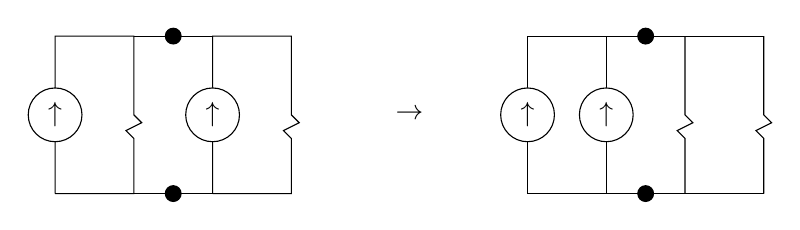
\begin{tikzpicture}
\draw (0,0)--(0,1)node[circle, draw=black, fill=white]{$\uparrow$}
--(0,2)--(1,2)--(1,1)--(1.1,.9)--(.9,.8)--(1,.7)--(1,0)--(0,0);
\draw (2,0)--(2,1)node[circle, draw=black, fill=white]{$\uparrow$}
--(2,2)--(3,2)--(3,1)--(3.1,.9)--(2.9,.8)--(3,.7)--(3,0)--(2,0);
\draw (2,0)--(1,0) (2,2)--(1,2);
\filldraw (1.5,0) circle[radius=1 mm];
\filldraw (1.5,2) circle[radius=1 mm];
\draw (6,0)--(6,1)node[circle, draw=black, fill=white]{$\uparrow$}--(6,2);
\draw (8,2)--(8,2)--(8,1)--(8.1,.9)--(7.9,.8)--(8,.7)--(8,0)--(8,0);
\draw (7,0)--(7,1)node[circle, draw=black, fill=white]{$\uparrow$}--(7,2);
\draw (9,2)--(9,2)--(9,1)--(9.1,.9)--(8.9,.8)--(9,.7)--(9,0)--(9,0);
\draw (9,0)--(6,0) (9,2)--(6,2);
\filldraw (7.5,0) circle[radius=1 mm];
\filldraw (7.5,2) circle[radius=1 mm];
\draw node at (4.5,1) {$\rightarrow$};
\end{tikzpicture}
\caption{Redrawing Parallel Norton Equivalents to make clear parallel combinations.}
\label{F:4STCOM}
\end{center}
\end{figure}

As we analyze circuits, we will look for situations when it is advantageous transform from Thevenin to Norton or visa versa.

\begin{blevel}
Consider two circuits, W and Y, that are in series. $W_T=(3V,10\Omega)$ and $Y_T=(-2V,2\Omega)$. Combine them and report the combined Thevenin equivalent. Draw the new circuit.
\end{blevel}

\begin{clevel}
Consider two circuits, W and Y, that are in series. $W_N=(3A,10\Omega)$ and $Y_T=(-2V,2\Omega)$. Combine them and report the combined Thevenin equivalent. Draw the new circuit.
\end{clevel}

%%%%%%%%%%%%%%%%%%%%%%%%%%%%%%%%%%%%%%%%%%%%
\subsection{Source Transformation Example}
Let's find the current through the 2 Ohm resistor for the circuit shown in Figure~\ref{F:4STEX}. Look at the circuit diagram and try to identify some Th\'{e}venin and Norton sources.

\begin{figure}[H]
\begin{center}
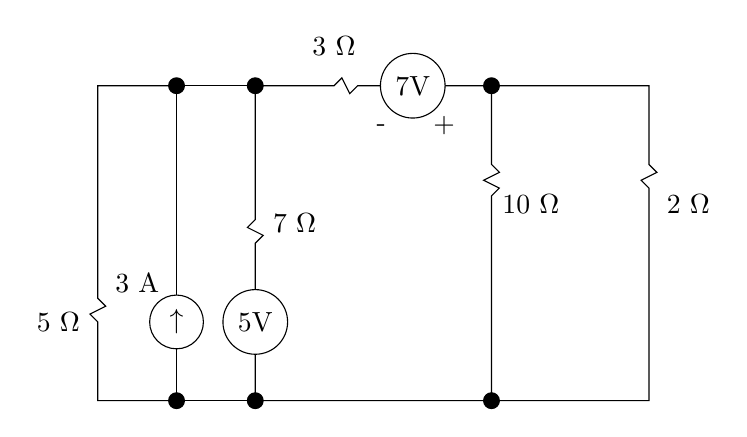
\begin{tikzpicture}
\draw (0,0)--(-1,0)--(-1,1)--(-1.1,1.1)--(-.9,1.2)--(-1,1.3)--(-1,4)--(0,4);
\draw (1,0)--(0,0)--(0,1) node[circle, draw=black, fill=white]{$\uparrow$}--(0,4)--(1,4);
\draw (1,0)--(1,1) node[circle, draw=black, fill=white]{5V}--
(1,2)--(1.1,2.1)--(.9,2.2)--(1,2.3)--(1,4);
\filldraw (1,0) circle[radius=1 mm];
\filldraw (1,4) circle[radius=1 mm];
\filldraw (4,4) circle[radius=1 mm];
\filldraw (0,4) circle[radius=1 mm];
\filldraw (0,0) circle[radius=1 mm];
\filldraw (4,0) circle[radius=1 mm];
\draw node at (-.5,1.5) {3 A};
\draw node at (-1.5,1) {5 $\Omega$};
\draw node at (1.5,2.25) {7 $\Omega$};
\draw node at (2,4.5) {3 $\Omega$};
\draw node at (6.5,2.5) {2 $\Omega$};
\draw node at (4.5,2.5) {10 $\Omega$};
\draw (1,4)--(2,4)--(2.1,4.1)--(2.2,3.9)--(2.3,4)--(3,4)node[circle, draw=black,fill=white]{7V}--(4,4);
\draw node at (3.4,3.5){+};
\draw node at (2.6,3.5){-};
\draw (4,4)--(4,3)--(4.1,2.9)--(3.9,2.8)--(4.1,2.7)--(4,2.6)--(4,0)--(1,0);
\draw (4,4)--(6,4)--(6,3)--(6.1,2.9)--(5.9,2.8)--(6,2.7)--(6,0)--(4,0);
\end{tikzpicture}
\caption{Source transformation example. Unsimplified circuit.}
\label{F:4STEX}
\end{center}
\end{figure}

Figure~\ref{F:4STEXID} identifies some Thevenin and Norton combinations and labels them A,B,C and D. Maybe the most surprising is D. While just a resistor, it's equivalent to a resistor in series with a 0V source\footnote{Or in parallel with a 0 Amp current source.}.

\begin{figure}[H]
\begin{center}
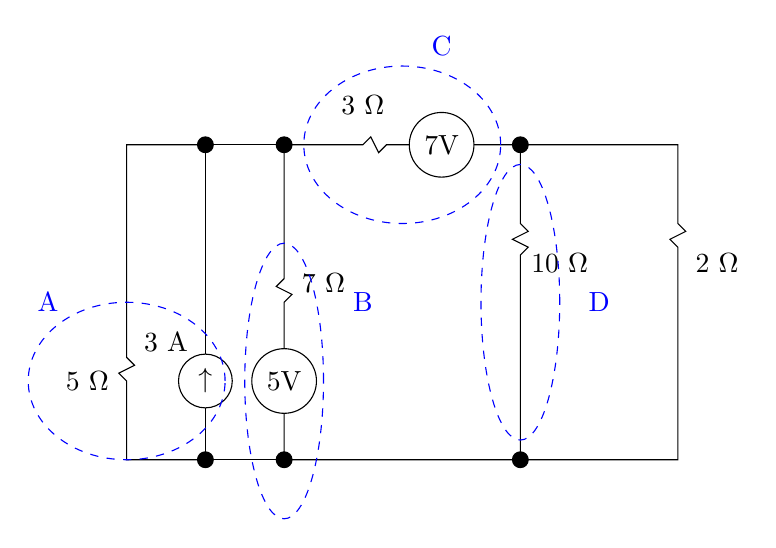
\begin{tikzpicture}
\draw (0,0)--(-1,0)--(-1,1)--(-1.1,1.1)--(-.9,1.2)--(-1,1.3)--(-1,4)--(0,4);
\draw (1,0)--(0,0)--(0,1) node[circle, draw=black, fill=white]{$\uparrow$}--(0,4)--(1,4);
\draw (1,0)--(1,1) node[circle, draw=black, fill=white]{5V}--
(1,2)--(1.1,2.1)--(.9,2.2)--(1,2.3)--(1,4);
\filldraw (1,0) circle[radius=1 mm];
\filldraw (1,4) circle[radius=1 mm];
\filldraw (4,4) circle[radius=1 mm];
\filldraw (0,4) circle[radius=1 mm];
\filldraw (0,0) circle[radius=1 mm];
\filldraw (4,0) circle[radius=1 mm];
\draw node at (-.5,1.5) {3 A};
\draw node at (-1.5,1) {5 $\Omega$};
\draw node at (1.5,2.25) {7 $\Omega$};
\draw node at (2,4.5) {3 $\Omega$};
\draw node at (6.5,2.5) {2 $\Omega$};
\draw node at (4.5,2.5) {10 $\Omega$};
\draw (1,4)--(2,4)--(2.1,4.1)--(2.2,3.9)--(2.3,4)--(3,4)node[circle, draw=black,fill=white]{7V}--(4,4);
\draw (4,4)--(4,3)--(4.1,2.9)--(3.9,2.8)--(4.1,2.7)--(4,2.6)--(4,0)--(1,0);
\draw (4,4)--(6,4)--(6,3)--(6.1,2.9)--(5.9,2.8)--(6,2.7)--(6,0)--(4,0);
\draw [dashed, draw=blue] (2.5,4) ellipse (1.25 cm and 1 cm);
\draw [dashed, draw=blue] (-1,1) ellipse (1.25 cm and 1 cm);
\draw [dashed, draw=blue] (1,1) ellipse (.5 cm and 1.75 cm);
\draw [dashed, draw=blue] (4,2) ellipse (.5 cm and 1.75 cm);
\draw node[text=blue] at (-2,2) {A};
\draw node[text=blue] at (2.,2) {B};
\draw node[text=blue] at (3,5.25) {C};
\draw node[text=blue] at (5,2) {D};
\end{tikzpicture}
\caption{Source transformation example with strategy identified.}
\label{F:4STEXID}
\end{center}
\end{figure}

Sources A and B are in parallel. That combination is in series with source C. That total combination is in parallel with source D. That whole mess is then both in series and/or parallel with the 2 Ohm resistor. We can distill all that into this expression:\\

\begin{align}
\text{circuit (excluding 2 Ohm)} =((A \parallel B)+C) \parallel D)
\end{align}

Now let's work out the details:

\begin{enumerate}
\item To combine A and B in parallel, they should both be Norton equivalents. $A_N=(3A,5\Omega)$ and $B_N=(\frac{5}{7}A,7\Omega)$. Combined $(A\parallel B)_N=(3\frac{5}{7}A,\frac{35}{12}\Omega)$.
\item To combine $(A \parallel B)$ in series with C, it should both be written as a  Thevenin equivalent: $(A \parallel B)_T = (10.83V, \frac{35}{12}\Omega)$ and $C_T=(7V,3\Omega)$. This gives $(A \parallel B)_T+C_T = (17.83V,5.92\Omega)$.
\item To combine this in parallel with D, go back to the Norton version. $((A \parallel B)+C)_N = (3.014A,5.92\Omega)$, and $D_N=(0A, 10\Omega)$. Combined gives, $((A \parallel B)+C)\parallel D)_N=(3.014A,3.72\Omega)$.
\item Taking this back to Th\'{e}venin format: $((A \parallel B)+C)\parallel D)_T=(11.2V,3.72\Omega)$.
\item Now the circuit looks like Figure~\ref{F:Simplified} and the current through the $2 \Omega$ resistor can be calculated to be $\frac{11.2V}{5.72\Omega} = 1.97 A$. Done.
\end{enumerate}

\begin{figure}[H]
\begin{center}
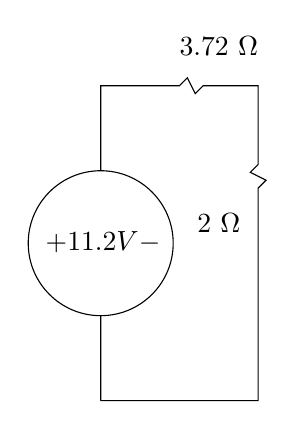
\begin{tikzpicture}
\draw (0,0)--(0,2) node[circle, draw=black, fill=white]{$\begin{matrix}+\\11.2V\\-\end{matrix}$}--(0,4)--(1,4)
--(1.1,4.1)--(1.2,3.9)--(1.3,4)--(2,4)
--(2,3)--(1.9,2.9)--(2.1,2.8)--(2,2.7)--(2,0)--(0,0);;
\draw node at (1.5,2.25) {2 $\Omega$};
\draw node at (1.5,4.5) {3.72 $\Omega$};
\end{tikzpicture}
\caption{Simplied Circuit after Source Transformations}
\label{F:Simplified}
\end{center}
\end{figure}

\begin{clevel}
Reconsider Figure~\ref{F:4STEX}. This time use the procedure to the determine the current through the 5 Ohm resistor. Start at the right side of the diagram and work your way to the left. Hint: Start by combining the 10 and 2 Ohm resistors in parallel and then in series with combo C.
\end{clevel}

%%%%%%%%%%%%%%%%%%%%%%%%%%%%%%%%%%%%%%%%%%%%%%%%%%%%%%%%%%
\section{Superposition and Linearity}
\textbf{A Superposition Situation:} Imagine you work at a coffee shop. While you work, the shop sells \$60 of coffee per hour. A different employee, J, working a different shift, sells \$50 of coffee per hour. The shop considers having you both work at the same time. Do you suppose the shop will sell \$110 of coffee?\\
\\
If the coffee shop behaves as a \textbf{linear system}, then together you would earn \$110. The contributions of you and J can be added (superimposed) together.
\par
Let's capture this idea with an equation (`I' represents the coffee shop's income):

\begin{align*}
I(you+J) = I(you)+I(J)
\end{align*}

Or more generally\footnote{For linear systems, the claim is often written as: $f(\alpha x,\beta y) = \alpha f(x)+\beta f(y)$.},

\begin{align}
f(x+y) = f(x)+f(y) \label{E:4LIN}
\end{align}

Note that for a linear system it would follow that, 
\begin{align*}
f(x+x) &= f(x)+f(x) \\
f(2x)&=2f(x)
\end{align*}
Maybe you can convince yourself that $f(kx)=kf(x)$.\par

\begin{alevel}
How much income would the coffee shop make per hour if two clones of you were to work at the same time? Assume superposition holds.
\end{alevel}

\begin{bigidea} Many engineering systems can be approximated as linear systems.
\end{bigidea}

Equation~\eqref{E:4LIN} does not usually exactly apply\footnote{Remember, Ohm's Law is just an approximation.}, but in many cases, linearity applies closely enough that\footnote{Sometimes not even that closely!} the mathematical benefit makes the linearity assumption worthwhile.
\par
\textbf{Claim:} If a circuit contains only voltage/current sources and resistors, then the circuit will behave as a linear system. \par
Imagine a circuit with three sources and one output voltage of interest, $V_{out}$. $V_{out}$ would be some function of the three sources, $S_1,S_2,S_3$.
\par
\begin{align}
V_{out} = f(S_1,S_2,S_3)
\end{align}

If the system is linear, then:
\par
\begin{align}
V_out &= f(S_1,S_2,S_3) \notag\\
	&= f(S_1,0,0)+f(0,S_2,0)+f(0,0,S_3) \label{E:4LIN2}
\end{align}

The zeros indicate that source has been turned off (0V for a voltage source, or 0 Amps for a current source). This would also be true, but probably not as useful:
\par
\begin{align}
V_out &= f(S_1,S_2,S_3) \\
	&= f(S_1,4S_2,.5S_3)+f(0,-3S_2,0)+f(0,0,0.5S_3)
\end{align}

We plan to determine $V_{out}$ by summing together the individual contributions due to each source, with the other sources turned off. In other words, we'll use Equation~\eqref{E:4LIN2}. To turn off a power source:\

\begin{itemize}
\item If it's a voltage source, set the voltage to zero by replacing it with the short circuit (an open circuit could still have a voltage difference across it).
\item If it's a current source, make the current through it zero by replacing it with an open circuit (a short circuit could still have current through it)
\end{itemize}

\begin{blevel}
A linear circuit has two sources, a 5A current source and a 3V voltage source. The output due to just the 5A current source is 3.5V and the output due to just the 3V source is 17 Volts. What will the output be with both sources on at the same time?
\end{blevel}

\begin{clevel}
A linear circuit has two sources, a 5A current source and a 3V voltage source. The output due to just the 5A current source is 3.5V and the output due to just the 3V source is 17 Volts. What will the output be with the current source set to 10A and the voltage source set to 9V?
\end{clevel}

\begin{alevel}
For the coffee shop, what would be:
\begin{align*}
I(0.5*you,3*Friend)=?\\
I(0,3*Friend)+I(0.5*you,0)=?
\end{align*}
\end{alevel}

%%%%%%%%%%%%%%%%%%%%%%%%%%%%%%%%%%
\subsection{Superposition Example}
Let's try an example like the Figure~\ref{F:4NODV}. The output voltage ($V_{out}$) will be the voltage drop across the 5 $\Omega$ resistor ($V_{DA}$).

\begin{figure}[H]
\begin{center}
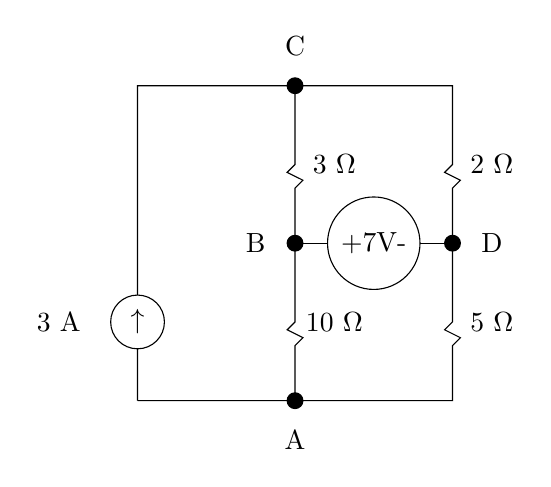
\begin{tikzpicture}
\draw (0,0)--(0,1)node[circle, draw=black, fill=white]{$\uparrow$}--(0,4)--(2,4)--(2,3)
--(1.9,2.9)--(2.1,2.8)--(2,2.7)--(2,2)--(2,1)
--(1.9,.9)--(2.1,.8)--(2,.7)--(2,0)--(0,0);
\draw (2,4)--(4,4)--(4,3)
--(3.9,2.9)--(4.1,2.8)--(4,2.7)--(4,2);
\draw (2,2)--(3,2)node[circle, draw=black, fill=white]{+7V-}--(4,2);
\draw (4,2)--(4,1)
--(3.9,.9)--(4.1,.8)--(4,.7)--(4,0)--(2,0);
\draw node at (-1,1) {3 A};
\draw node at (2.5,1) {10 $\Omega$};
\draw node at (4.5,1) {5 $\Omega$};
\draw node at (2.5,3) {3 $\Omega$};
\draw node at (4.5,3) {2 $\Omega$};
\draw node at (1.5,2) {B};
\draw node at (2,-.5) {A};
\draw node at (2,4.5) {C};
\draw node at (4.5,2) {D};
\filldraw (2,4) circle[radius=1 mm];
\filldraw (2,2) circle[radius=1 mm];
\filldraw (4,2) circle[radius=1 mm];
\filldraw (2,0) circle[radius=1 mm];
\end{tikzpicture}
\caption{Superposition example}
\end{center}
\end{figure}

The principle of superposition says that $V_{out}$ depends on the 3A current source (with the 7V source shorted) and the 7V source with the 3A current source as an open circuit. We'll structure our answer so that we don't lose track:

\begin{align*}
V_{out}(3A, 7V)&=V_{out}(3A,0)+V_{out}(0, 7V)\\
V_{out}&=\underbrace{\rule{1 cm}{.25 mm}}_{3A}+\underbrace{\rule{1 cm}{.25 mm}}_{7V}
\end{align*}

First, with the 7V source shorted:

\begin{figure}[H]
\begin{center}
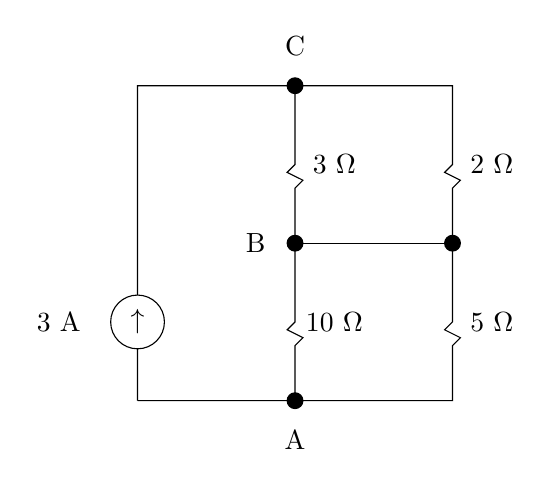
\begin{tikzpicture}
\draw (0,0)--(0,1)node[circle, draw=black, fill=white]{$\uparrow$}--(0,4)--(2,4)--(2,3)
--(1.9,2.9)--(2.1,2.8)--(2,2.7)--(2,2)--(2,1)
--(1.9,.9)--(2.1,.8)--(2,.7)--(2,0)--(0,0);
\draw (2,4)--(4,4)--(4,3)
--(3.9,2.9)--(4.1,2.8)--(4,2.7)--(4,2);
\draw (2,2)--(3,2)--(4,2);
\draw (4,2)--(4,1)
--(3.9,.9)--(4.1,.8)--(4,.7)--(4,0)--(2,0);
\draw node at (-1,1) {3 A};
\draw node at (2.5,1) {10 $\Omega$};
\draw node at (4.5,1) {5 $\Omega$};
\draw node at (2.5,3) {3 $\Omega$};
\draw node at (4.5,3) {2 $\Omega$};
\draw node at (1.5,2) {B};
\draw node at (2,-.5) {A};
\draw node at (2,4.5) {C};
%\draw node at (4.5,2) {D};
\filldraw (2,4) circle[radius=1 mm];
\filldraw (2,2) circle[radius=1 mm];
\filldraw (4,2) circle[radius=1 mm];
\filldraw (2,0) circle[radius=1 mm];
\end{tikzpicture}
\caption{Superposition example with 7V source (turned off) shorted.}
\end{center}
\end{figure}

Solving for $V_{out}$ still takes several steps:

\begin{enumerate}
\item Observe that B and D are now the same node (they are connected by a perfect wire).
\item Observe that the 3 and 2 Ohm resistors are in parallel, as are the 10 and 5 Ohm resistors.
\item Combine the two parallel combinations to get:
\begin{align*}
R_{CB}=3\parallel 2=1.2 \Omega && R_{BA}=10\parallel 5=3.33 \Omega
\end{align*}

\item The current source forces 3A through both the 1.2 and 3.33 $\Omega$ resistors. A voltage drop $V_{BA}$ results: $V_{BA}=IR=3*3.33 = 10V$.
\end{enumerate}

Then, with the 7V source turned back on and the 3A current source set to zero (disconnected):

\begin{figure}[H]
\begin{center}
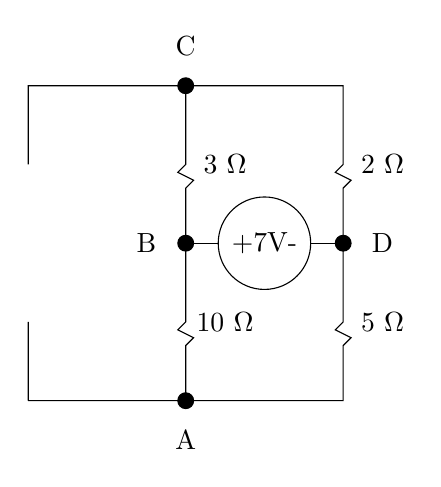
\begin{tikzpicture}
\draw (0,0)--(0,1) (0,3)--(0,4)--(2,4)--(2,3)
--(1.9,2.9)--(2.1,2.8)--(2,2.7)--(2,2)--(2,1)
--(1.9,.9)--(2.1,.8)--(2,.7)--(2,0)--(0,0);
\draw (2,4)--(4,4)--(4,3)
--(3.9,2.9)--(4.1,2.8)--(4,2.7)--(4,2);
\draw (2,2)--(3,2)node[circle, draw=black, fill=white]{+7V-}--(4,2);
\draw (4,2)--(4,1)
--(3.9,.9)--(4.1,.8)--(4,.7)--(4,0)--(2,0);
%\draw node at (-1,1) {3 A};
\draw node at (2.5,1) {10 $\Omega$};
\draw node at (4.5,1) {5 $\Omega$};
\draw node at (2.5,3) {3 $\Omega$};
\draw node at (4.5,3) {2 $\Omega$};
\draw node at (1.5,2) {B};
\draw node at (2,-.5) {A};
\draw node at (2,4.5) {C};
\draw node at (4.5,2) {D};
\filldraw (2,4) circle[radius=1 mm];
\filldraw (2,2) circle[radius=1 mm];
\filldraw (4,2) circle[radius=1 mm];
\filldraw (2,0) circle[radius=1 mm];
\end{tikzpicture}
\caption{Superposition example with 3A source turned off (open circuit)}
\end{center}
\end{figure}

Observe that the 5 and 10 $\Omega$ resistors are now in series. By voltage division, the voltage across the 5 Ohm resistor is \footnote{Path BCD did not matter.}:
\begin{align*}
V_{DA}=\frac{5}{10+5}(-7V)=-2.33V
\end{align*}

Putting the two pieces together gives:

\[
V_{out}=\underbrace{\underline{10V}}_{3A}+\underbrace{\underline{-2.33V}}_{7V} = 7.66V
\]

\begin{blevel}
Suppose we increased the 7V source to 14V. What would the output voltage be?
\end{blevel}

\begin{clevel}
Suppose the current source and voltage source were to switch positions. Redo the superposition analysis to determine $V_{out}$.
\end{clevel}

\subsection{Superposition in Engineering Statics}
Consider a 5 kg beam (10 feet long) resting on two supports as shown. There is also a 10 kg menhir resting on the beam such that its center rests 7 feet from the left side. Use superposition to determine the force of the right support pushing upwards on the beam.
\par
\[
F=\underbrace{\rule{1 cm}{.25 mm}}_{F_{beam}}+\underbrace{\rule{1 cm}{.25 mm}}_{F_{menhir}}
\]

\begin{figure}[H]
\begin{center}
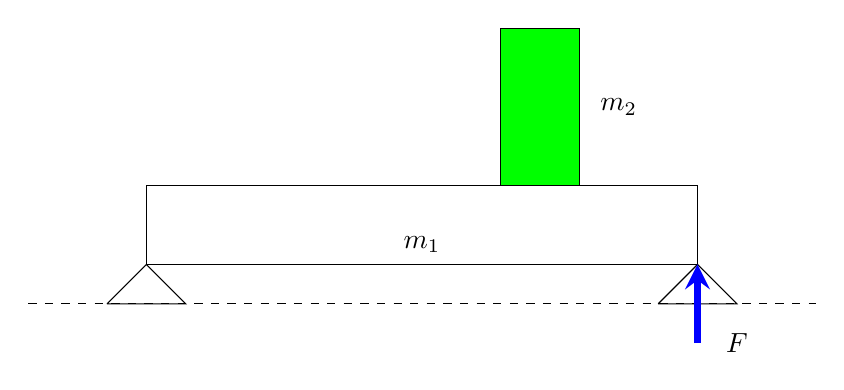
\begin{tikzpicture}
\draw [dashed] (-1,.5)--(9,.5);
\draw (0,.5)--(.5,1)-- (1,.5)--(0,.5);
\draw (7,.5)--(7.5,1)-- (8,.5)--(7,.5);
\draw (.5,1) rectangle (7.5,2);
\draw [draw=black, fill=green] (5,2) rectangle (6,4);
\draw [draw=blue, line width = 1mm] [-stealth](7.5,0)--(7.5,1);
\draw node at (6.5,3) {$m_2$};
\draw node at (4,1.25) {$m_1$};
\draw node at (8,0) {$F$};
\end{tikzpicture}
\caption{Superposition in mechanics. Determine F.}
\end{center}
\end{figure}

First, find the contribution due to $m_1$. By symmetry, it must be half the weight of the beam. Half of 49N is 24.5N.

Second, find the contribution due to the menhir ($m_2$) only (treating the beam as massless). We'll set the sum of the moments about the left side to be zero.
\par
\begin{align*}
\text{Sum of Moments about Left Side: }&&\sum{M_{LEFT}}=-98*7+F*10=0\\
&&F=68.6N
\end{align*}

Therefore, the total force on the right side would be:

\[
F=\underbrace{\underline{24.5N}}_{F_{beam}}+\underbrace{\underline{68.5N}}_{F_{menhir}}
\]
\begin{align*}
F=93N
\end{align*}

\begin{blevel}
What would be the force F if the menhir doubled in weight?
\end{blevel}

\begin{clevel}
What would be the force F if the beam's weight were changed to 16kg and the menhir to 25 kg?
\end{clevel}


%%%%%%%%%%%%%%%%%%%%%%%%%%%%%%%%%%%%%%%%%%%%%%%%%%%%%%%%%%%%
\section{A circuit solved by all four techniques}
We return now to the circuit we used to demonstrate the source transformation technique. In this section we check our work by solving the same circuit using all four methods.

\begin{figure}[H]
\begin{center}
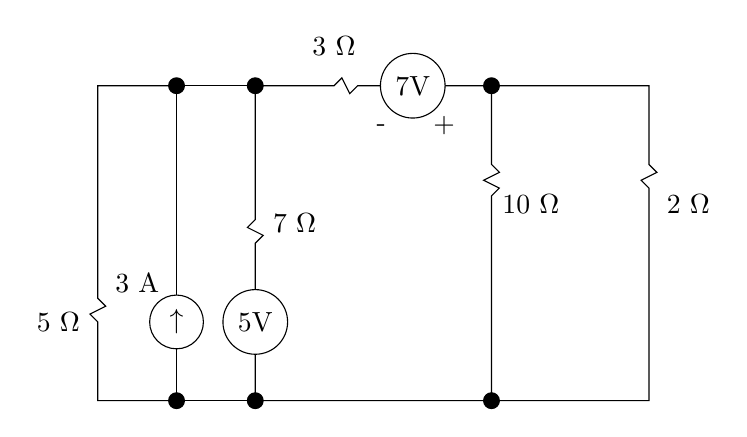
\begin{tikzpicture}
\draw (0,0)--(-1,0)--(-1,1)--(-1.1,1.1)--(-.9,1.2)--(-1,1.3)--(-1,4)--(0,4);
\draw (1,0)--(0,0)--(0,1) node[circle, draw=black, fill=white]{$\uparrow$}--(0,4)--(1,4);
\draw (1,0)--(1,1) node[circle, draw=black, fill=white]{5V}--
(1,2)--(1.1,2.1)--(.9,2.2)--(1,2.3)--(1,4);
\filldraw (1,0) circle[radius=1 mm];
\filldraw (1,4) circle[radius=1 mm];
\filldraw (4,4) circle[radius=1 mm];
\filldraw (0,4) circle[radius=1 mm];
\filldraw (0,0) circle[radius=1 mm];
\filldraw (4,0) circle[radius=1 mm];
\draw node at (-.5,1.5) {3 A};
\draw node at (-1.5,1) {5 $\Omega$};
\draw node at (1.5,2.25) {7 $\Omega$};
\draw node at (2,4.5) {3 $\Omega$};
\draw node at (6.5,2.5) {2 $\Omega$};
\draw node at (4.5,2.5) {10 $\Omega$};
\draw (1,4)--(2,4)--(2.1,4.1)--(2.2,3.9)--(2.3,4)--(3,4)node[circle, draw=black,fill=white]{7V}--(4,4);
\draw node at (3.4,3.5){+};
\draw node at (2.6,3.5){-};
\draw (4,4)--(4,3)--(4.1,2.9)--(3.9,2.8)--(4.1,2.7)--(4,2.6)--(4,0)--(1,0);
\draw (4,4)--(6,4)--(6,3)--(6.1,2.9)--(5.9,2.8)--(6,2.7)--(6,0)--(4,0);
\end{tikzpicture}
\caption{Circuit to be solved by all four methods.}
\end{center}
\end{figure}

%%%%%%%%%%%%%%%%%%%%%%%%%%%%%
\subsection{Nodal Analysis}
Identify the nodes - there are five. Set one as the reference node (use A=0). Label currents through voltage sources - there are two of these ($I_1$ and $I_2$).

\begin{figure}[H]
\begin{center}
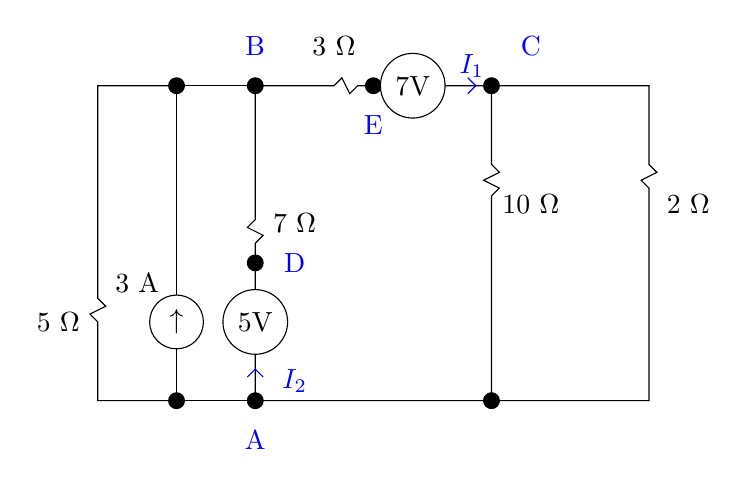
\begin{tikzpicture}
\draw (0,0)--(-1,0)--(-1,1)--(-1.1,1.1)--(-.9,1.2)--(-1,1.3)--(-1,4)--(0,4);
\draw (1,0)--(0,0)--(0,1) node[circle, draw=black, fill=white]{$\uparrow$}--(0,4)--(1,4);
\draw (1,0)--(1,1) node[circle, draw=black, fill=white]{5V}--
(1,2)--(1.1,2.1)--(.9,2.2)--(1,2.3)--(1,4);
\filldraw (1,0) circle[radius=1 mm];
\filldraw (1,4) circle[radius=1 mm];
\filldraw (4,4) circle[radius=1 mm];
\filldraw (0,4) circle[radius=1 mm];
\filldraw (0,0) circle[radius=1 mm];
\filldraw (4,0) circle[radius=1 mm];
\draw node at (-.5,1.5) {3 A};
\draw node at (-1.5,1) {5 $\Omega$};
\draw node at (1.5,2.25) {7 $\Omega$};
\draw node at (2,4.5) {3 $\Omega$};
\draw node at (6.5,2.5) {2 $\Omega$};
\draw node at (4.5,2.5) {10 $\Omega$};
\draw node[text=blue] at (1,-.5) {A};
\draw node[text=blue] at (1,4.5) {B};
\draw node[text=blue] at (4.5,4.5) {C};
\draw node[text=blue] at (1.5,1.75) {D};
\draw node[text=blue] at (2.5,3.5) {E};
\filldraw (1,1.75) circle[radius=1 mm];
\filldraw (2.5,4) circle[radius=1 mm];
\draw (1,4)--(2,4)--(2.1,4.1)--(2.2,3.9)--(2.3,4)--(3,4)node[circle, draw=black,fill=white]{7V}--(4,4);
\draw (4,4)--(4,3)--(4.1,2.9)--(3.9,2.8)--(4.1,2.7)--(4,2.6)--(4,0)--(1,0);
\draw (4,4)--(6,4)--(6,3)--(6.1,2.9)--(5.9,2.8)--(6,2.7)--(6,0)--(4,0);
\draw [draw=blue] (3.7,4.1)--(3.8,4)--(3.7,3.9);
\draw node[text=blue] at (3.75,4.25) {$I_1$};
\draw [draw=blue] (.9,.3)--(1,.4)--(1.1,.3);
\draw node[text=blue] at (1.5,.25) {$I_2$};
\end{tikzpicture}
\caption{With Nodes identified. Set A as the reference.}
\end{center}
\end{figure}

Write down node equations for the non-reference nodes. \footnote{You could skip Node D we know it must be 5V above reference. If one side of a voltage source is attached to reference, then you know the voltage at the other end.}

\begin{align*}
\text{Node B: }&\frac{0-B}{5}+3+\frac{D-B}{7}+\frac{E-B}{3}=0\\
\text{Node C: }&I_1+\frac{0-C}{10}+\frac{0-C}{2}=0\\
\text{Node D: }&\frac{B-D}{7}+I_2=0\\
\text{Node E: }&\frac{B-E}{3}-I_1=0\\
\text{Bonus 5V Source: }&D=0+5\\
\text{Bonus 7V Source: }&C=E+7
\end{align*}

In matrix form:

\begin{align*}
\left[ \begin{matrix}
(-\frac{1}{5}-\frac{1}{7}-\frac{1}{3})	&0	&\frac{1}{7}	&\frac{1}{3} &0&0\\
0	&(-\frac{1}{10}-\frac{1}{2})	&0	&0	&1&0\\
\frac{1}{7}	&0	&(-\frac{1}{7}) &0	&0	&1\\
\frac{1}{3}	&0	&0	&(-\frac{1}{3})	&-1	&0\\
0	&0	&1	&0	&0	&0\\
0	&1	&0	&-1	&0	&0\\
\end{matrix} \right]
\left[ \begin{matrix}
B\\
C\\
D\\
E\\
I_1\\
I_2
\end{matrix} \right] =
\left[ \begin{matrix}
-3\\
0\\
0\\
0\\
5\\
7
\end{matrix} \right]
\end{align*}

Solving gives C = 3.92 V. This represents the voltage difference between node C and the reference, node A. Finally, find the current through the 2 Ohm resistor by dividing the voltage drop across it by its resistance (2 $\Omega$). Result: I= 1.96 A.
\par
\subsection{Loop Analysis}
Identify the loops. There are four. Also, notice the current source. The voltage across it is unknown so we'll label the voltage drop across it as $V_1$ 

\begin{figure}[H]
\begin{center}
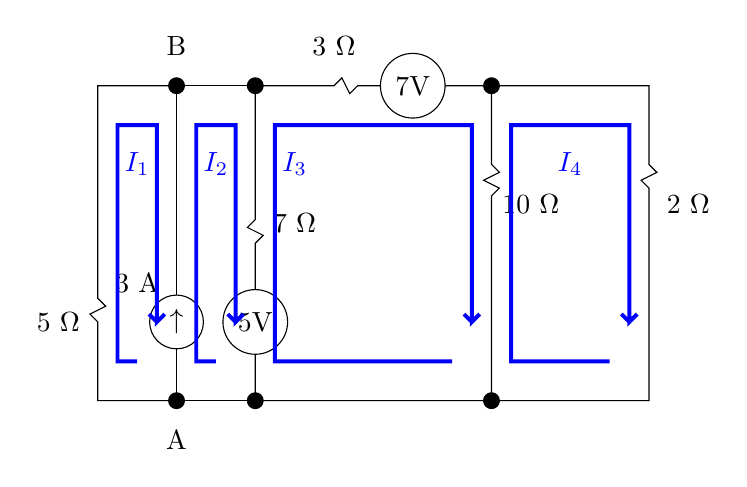
\begin{tikzpicture}
\draw (0,0)--(-1,0)--(-1,1)--(-1.1,1.1)--(-.9,1.2)--(-1,1.3)--(-1,4)--(0,4);
\draw (1,0)--(0,0)--(0,1) node[circle, draw=black, fill=white]{$\uparrow$}--(0,4)--(1,4);
\draw (1,0)--(1,1) node[circle, draw=black, fill=white]{5V}--
(1,2)--(1.1,2.1)--(.9,2.2)--(1,2.3)--(1,4);
\filldraw (1,0) circle[radius=1 mm];
\filldraw (1,4) circle[radius=1 mm];
\filldraw (4,4) circle[radius=1 mm];
\filldraw (0,4) circle[radius=1 mm];
\filldraw (0,0) circle[radius=1 mm];
\filldraw (4,0) circle[radius=1 mm];
\draw node at (-.5,1.5) {3 A};
\draw node at (-1.5,1) {5 $\Omega$};
\draw node at (1.5,2.25) {7 $\Omega$};
\draw node at (2,4.5) {3 $\Omega$};
\draw node at (6.5,2.5) {2 $\Omega$};
\draw node at (4.5,2.5) {10 $\Omega$};
\draw node at (0,4.5) {B};
\draw node at (0,-.5) {A};
\draw (1,4)--(2,4)--(2.1,4.1)--(2.2,3.9)--(2.3,4)--(3,4)node[circle, draw=black,fill=white]{7V}--(4,4);
\draw (4,4)--(4,3)--(4.1,2.9)--(3.9,2.8)--(4.1,2.7)--(4,2.6)--(4,0)--(1,0);
\draw (4,4)--(6,4)--(6,3)--(6.1,2.9)--(5.9,2.8)--(6,2.7)--(6,0)--(4,0);
\draw [draw=blue, line width=0.5mm] (-.5,.5)--(-.75,.5)--(-.75,3.5)
--(-.25,3.5)--(-.25,1)--(-.15,1.1)--(-.25,1)--(-.35,1.1);
\draw [text=blue] node at (-.5,3) {$I_1$};
\draw [draw=blue, line width=0.5mm] (.5,.5)--(.25,.5)--(.25,3.5)
--(.75,3.5)--(.75,1)--(.85,1.1)--(.75,1)--(.65,1.1);
\draw [text=blue] node at (.5,3) {$I_2$};
\draw [draw=blue, line width=0.5mm] (3.5,.5)--(1.25,.5)--(1.25,3.5)
--(3.75,3.5)--(3.75,1)--(3.85,1.1)--(3.75,1)--(3.65,1.1);
\draw [text=blue] node at (1.5,3) {$I_3$};
\draw [draw=blue, line width=0.5mm] (5.5,.5)--(4.25,.5)--(4.25,3.5)
--(5.75,3.5)--(5.75,1)--(5.85,1.1)--(5.75,1)--(5.65,1.1);
\draw [text=blue] node at (5,3) {$I_4$};
\end{tikzpicture}
\caption{With loops identified}
\end{center}
\end{figure}

Writing out KVL for each loop.

\begin{align*}
\text{Loop 1: }&&-5I_1-V_1&=0\\
\text{Loop 2: }&&V_1-7(I_2-I_3)-5&=0\\
\text{Loop 3: }&&5-7(I_3-I_2)-3I_3+7-10(I_3-I_4)&=0\\
\text{Loop 4: }&&-10(I_4-I_3)-2I_4&=0\\
\text{Bonus 3A Source: }&&I_2-I_1&=3
\end{align*}

In matrix form:

\begin{align*}
\left[ \begin{matrix}
-5	&0	&0	&0 &-1\\
0	&-7	&7	&0	&1\\
0	&7	&(-7-3-10) &10	&0\\
0	&0	&10	&(-10-2)	&0\\
-1	&1	&0	&0	&0	\\
\end{matrix} \right]
\left[ \begin{matrix}
I_1\\
I_2\\
I_3\\
I_4\\
V_1
\end{matrix} \right] =
\left[ \begin{matrix}
0\\
5\\
-5-7\\
0\\
3
\end{matrix} \right]
\end{align*}

Solving for $I_4$ gives the current through the 2 $\Omega$ resistor to be 1.96 A.

%%%%%%%%%%%%%%%%%%%%%%%%%%%%%%%%%%%
\subsection{Source Transformations}
This example was already completed. The answer was 1.96 A.

%%%%%%%%%%%%%%%%%%%%%%%%%%%5
\subsection{Superposition}
Because the circuit has three sources, our answer will have three parts:

\begin{align}
I_{2\Omega}=\underbrace{\rule{1 cm}{.25 mm}}_{3A}+\underbrace{\rule{1 cm}{.25 mm}}_{5V}
+\underbrace{\rule{1 cm}{.25 mm}}_{7V}
\end{align}


For the first part, shut off the other two sources. The network looks like this:
\begin{figure}[H]
\begin{center}
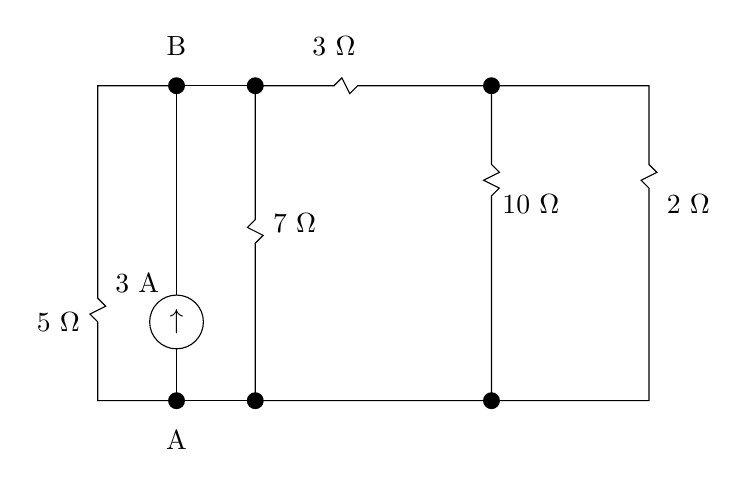
\begin{tikzpicture}
\draw (0,0)--(-1,0)--(-1,1)--(-1.1,1.1)--(-.9,1.2)--(-1,1.3)--(-1,4)--(0,4);
\draw (1,0)--(0,0)--(0,1) node[circle, draw=black, fill=white]{$\uparrow$}--(0,4)--(1,4);
\draw (1,0)--(1,1)--
(1,2)--(1.1,2.1)--(.9,2.2)--(1,2.3)--(1,4);
\filldraw (1,0) circle[radius=1 mm];
\filldraw (1,4) circle[radius=1 mm];
\filldraw (4,4) circle[radius=1 mm];
\filldraw (0,4) circle[radius=1 mm];
\filldraw (0,0) circle[radius=1 mm];
\filldraw (4,0) circle[radius=1 mm];
\draw node at (-.5,1.5) {3 A};
\draw node at (-1.5,1) {5 $\Omega$};
\draw node at (1.5,2.25) {7 $\Omega$};
\draw node at (2,4.5) {3 $\Omega$};
\draw node at (6.5,2.5) {2 $\Omega$};
\draw node at (4.5,2.5) {10 $\Omega$};
\draw node at (0,4.5) {B};
\draw node at (0,-.5) {A};
\draw (1,4)--(2,4)--(2.1,4.1)--(2.2,3.9)--(2.3,4)--(3,4)--(4,4);
\draw (4,4)--(4,3)--(4.1,2.9)--(3.9,2.8)--(4.1,2.7)--(4,2.6)--(4,0)--(1,0);
\draw (4,4)--(6,4)--(6,3)--(6.1,2.9)--(5.9,2.8)--(6,2.7)--(6,0)--(4,0);
\end{tikzpicture}
\caption{Superposition. With 7V and 5V sources shut off.}
\end{center}
\end{figure}

We'll use the following steps to determine the current through the 2 $\Omega$ resistor (there are lots of other ways you might proceed).

\begin{enumerate}
\item Find total resistance seen by the 3A source. Answer:$(5 \parallel 7)\parallel (3+10 \parallel 2) = 1.795 \Omega$
\item Determine voltage across the 3A source: 5.385V
\item Determine currents through $7 \Omega$ and $5 \Omega$ resistors and subtract those from 3A. The remaining current through the 3 $\Omega$ resistor is: 1.154 A.
\item This current passes through $3 \Omega$ of resistance. The voltage dropped across the 3 $\Omega$ resistor is: +3.46V. 
\item Use KVL to determine voltage across $2 \Omega$: 5.385-3.46=1.923V.
\item Use Ohm's Law to determine current through $2 \Omega$: I = 0.962 A.
\end{enumerate}

Next, shut off the 3A and 7V sources and reexamine the network.

\begin{figure}[H]
\begin{center}
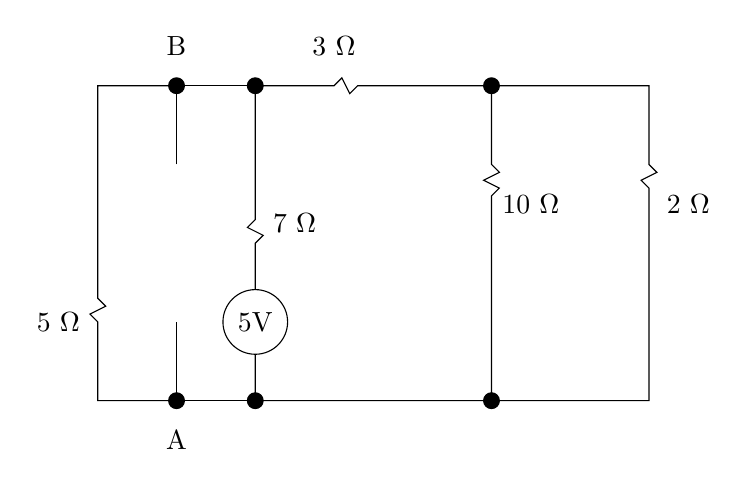
\begin{tikzpicture}
\draw (0,0)--(-1,0)--(-1,1)--(-1.1,1.1)--(-.9,1.2)--(-1,1.3)--(-1,4)--(0,4);
\draw (1,0)--(0,0)--(0,1) (0,3)--(0,4)--(1,4);
\draw (1,0)--(1,1) node[circle, draw=black, fill=white]{5V}--
(1,2)--(1.1,2.1)--(.9,2.2)--(1,2.3)--(1,4);
\filldraw (1,0) circle[radius=1 mm];
\filldraw (1,4) circle[radius=1 mm];
\filldraw (4,4) circle[radius=1 mm];
\filldraw (0,4) circle[radius=1 mm];
\filldraw (0,0) circle[radius=1 mm];
\filldraw (4,0) circle[radius=1 mm];
\draw node at (-1.5,1) {5 $\Omega$};
\draw node at (1.5,2.25) {7 $\Omega$};
\draw node at (2,4.5) {3 $\Omega$};
\draw node at (6.5,2.5) {2 $\Omega$};
\draw node at (4.5,2.5) {10 $\Omega$};
\draw node at (0,4.5) {B};
\draw node at (0,-.5) {A};
\draw (1,4)--(2,4)--(2.1,4.1)--(2.2,3.9)--(2.3,4)--(3,4)--(4,4);
\draw (4,4)--(4,3)--(4.1,2.9)--(3.9,2.8)--(4.1,2.7)--(4,2.6)--(4,0)--(1,0);
\draw (4,4)--(6,4)--(6,3)--(6.1,2.9)--(5.9,2.8)--(6,2.7)--(6,0)--(4,0);
\end{tikzpicture}
\caption{Superposition. With 7V and 3A sources shut off.}
\end{center}
\end{figure}

\begin{clevel}
Use a similar set of steps to show that the contribution to the current through the $2 \Omega$ resistor due to the 5V source is 0.229 A.
\end{clevel}

Finally, redraw the network with just the 7V supply.

\begin{figure}[H]
\begin{center}
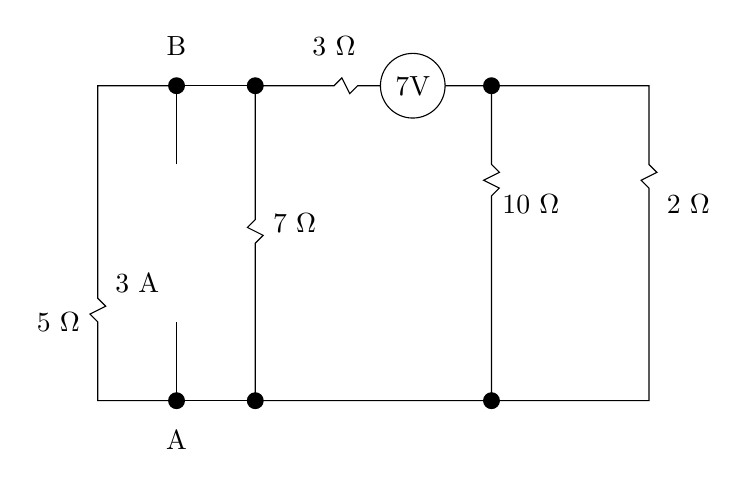
\begin{tikzpicture}
\draw (0,0)--(-1,0)--(-1,1)--(-1.1,1.1)--(-.9,1.2)--(-1,1.3)--(-1,4)--(0,4);
\draw (1,0)--(0,0)--(0,1) (0,3)--(0,4)--(1,4);
\draw (1,0)--(1,1)--
(1,2)--(1.1,2.1)--(.9,2.2)--(1,2.3)--(1,4);
\filldraw (1,0) circle[radius=1 mm];
\filldraw (1,4) circle[radius=1 mm];
\filldraw (4,4) circle[radius=1 mm];
\filldraw (0,4) circle[radius=1 mm];
\filldraw (0,0) circle[radius=1 mm];
\filldraw (4,0) circle[radius=1 mm];
\draw node at (-.5,1.5) {3 A};
\draw node at (-1.5,1) {5 $\Omega$};
\draw node at (1.5,2.25) {7 $\Omega$};
\draw node at (2,4.5) {3 $\Omega$};
\draw node at (6.5,2.5) {2 $\Omega$};
\draw node at (4.5,2.5) {10 $\Omega$};
\draw node at (0,4.5) {B};
\draw node at (0,-.5) {A};
\draw (1,4)--(2,4)--(2.1,4.1)--(2.2,3.9)--(2.3,4)--(3,4)node[circle, draw=black,fill=white]{7V}--(4,4);
\draw (4,4)--(4,3)--(4.1,2.9)--(3.9,2.8)--(4.1,2.7)--(4,2.6)--(4,0)--(1,0);
\draw (4,4)--(6,4)--(6,3)--(6.1,2.9)--(5.9,2.8)--(6,2.7)--(6,0)--(4,0);
\end{tikzpicture}
\caption{Superposition. With 3A and 5V sources shut off.}
\end{center}
\end{figure}

\begin{clevel}
Use a similar set of steps to show that the contribution to the current through the $2 \Omega$ resistor due to the 7V source is 0.769 A.
\end{clevel}

Our total current, using superposition, is then: 0.962A+0.229A+0.769A=1.96A.

\begin{align}
I_{2\Omega}=\underbrace{\underline{0.962A}}_{3A}+\underbrace{\underline{0.229A}}_{5V}
+\underbrace{\underline{0.769A}}_{7V} = 1.96A
\end{align}

Whew!

